\documentclass[12pt]{mcmthesis}
\mcmsetup{CTeX = false,   % 使用 CTeX 套装时,设置为 true
	tcn = 2002146, problem = D,
	sheet = true, titleinsheet = true, keywordsinsheet = true,
	titlepage = true}
\usepackage{palatino}
\usepackage{mwe}
\usepackage{graphicx}
\usepackage{subcaption}
\usepackage{float}
\usepackage{multirow}
\usepackage{indentfirst}
\usepackage{gensymb}
\usepackage[ruled,lined,commentsnumbered]{algorithm2e}
\usepackage{geometry}
\usepackage{pdfpages}
\begin{document}
	\linespread{0.6} %%行间距
	\setlength{\parskip}{0.5\baselineskip} %%段间距
	\title{iMoDs: A Treatment to the Kariba Dam}
	
	\date{\today}
	\begin{abstract}
		
		As the old saying goes, "If you want to go fast, go alone. If you want to go far, go together." Teamwork has become a more and more important part in our life. However, the best cooperation pattern is quite hard to be found. The complexity of human nature and the varieties of factors involved make even experts confused.
		
		Football, regarded as one of the most popular team sports in the world~c\cite{football}, is a perfect example of team work. To help our home football team, Huskies improve its performance, we has devised and implemented models to find out the particular factors that will help improve cooperation in the team. 
		
		We first build up a passing network and identify the network patterns. To be specific, we study the spatial and time distribution of passes during a game and modelling the team's attacking pattern by counting the forward passes. To avoid the drawback of treating the pass network merely as a static one, we format a \textbf{Time-varying model}, and study the variation of the network during the whole game. We study the changes in the pass-centroid and the formation of \textbf{triadic configurations}. 
		
		To study the indicators that reflect successful teamwork, we divided the aspects involved into two parts - the cooperation within the whole team and the performance of individual players. In the first part, we study the features of football-event network by checking its general features, as well as by looking further into some of its unique patterns. We study the total passing time, centroid of the passing network, clustering degree, maximum flow, connectivity and other patterns of the network to serve as hierarchical indicators for a team.
		
		In the second part, we build a Simulation-based model to evaluate the performance of each player in a game. In this model, we assume the shot number of each game as independent Poisson variables and assess their performance by adding up all the "contribution events".
		
		After normalizing the indicators mentioned above, we use Analytic Hierarchy Process(\textbf{AHP}) to help us find the weights of all the indicators found in the paper, and check its efficiency by comparing its results on different matches. Also in this part of work, we try to use Linear Regression(LR) to fit out the quantitative relationship between the indicator vector and the performance in a game. Considering the relatively high dimension of the indicator vectors, we use Principal Component Analysis(\textbf{PCA}) to make dimension reduction and try to make visualization of that relationship.
		
		In the next section, based on the results we get from the models, we give some \textbf{evaluations} of the current performance of the Huskies team. We also give some advice for the \textbf{strategies} in matching style, training players and improving cooperations to make Huskies a perform better in the next season. 
		
		To make our model more general, we extend the results from our model the serve a wider aspect of team work. We give emphasis on the team spirits, team member composition, assignment flow and keyman factor which we think play significant roles in other kind of team work in society. 
		
		Then we make sensitivity analysis of our model and find that our model is robust to the change of coefficients. 
		
		At the end of the paper, we list pros and cons of our model and make a conclusion of our work.
		
		\begin{keywords}
		Network analysis; Football player ranking; Analytic Hierarchy Process (AHP); Principal Component Analysis ({PCA}); Team cooperation
		\end{keywords}
	\end{abstract}
\maketitle

\tableofcontents

\newpage
\section{Introduction}
\subsection{Problem Background}
	As the social division of labor becomes more complex, team work has gained unprecedented importance. It becomes quite hard for anyone to achieve anything without help from others. However, the complexity of human nature and the varieties of factors involved means that the best cooperation pattern is hard to find. And team-sport is one of the fields that relies most on the effectiveness of cooperation. 
	
	\begin{figure}[h]
		\centering
		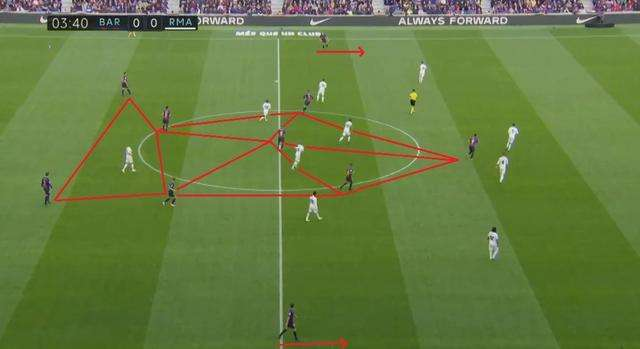
\includegraphics[width=0.5\textwidth]{tikitaka.jpg}
		\caption{Tiki-taka Strategy~\cite{tikitaka}}\label{fig:tiki}
	\end{figure}
	Football, as one of the most famous and complicated team sports, has attracted many people to enjoy its fantastic and changeful matches~\cite{football}. And the teamwork behind this game is also a rich field to be explored. For example, the F\'utbol Club Barcelona applied Tiki-taka, characterized by short passing and movement, in its matches. This strategy needs cooperation between football players and requires a lot of training. (Figure \ref{fig:tiki} shows the strategy.) It is useful to investigate the passing network of the ball between players to improve the strategy. Besides, to counter this strategy, the opponent team also needs to analyze their cooperation pattern and find out how to deal with its rival.
	
	To help improve the performance of our local football team, we are going to find out the key patterns that will make the football team great again. The results we get from the modelling can also be applied into other areas and help understand the key features for a successful team work in other fields.
	
\subsection{Interpretation of the Problem}
\begin{enumerate}
	\item We should create a network for the ball passing between players and analyze network patterns. We should consider both the micro part and the macro part.
	\item We should identify the factors that indicate the performance of the football team and build a model that captures numerous aspects of teamwork based on the factors.
	\item We should point out the strategies that have been effective for the specific football team and make out how they can improve their team performance later.
	\item We should generalize our findings to figure out how to design more effective team in the common daily teamwork, not just in a football team.
\end{enumerate}

\subsection{Our Work}
Figure \ref{fig:ourwork} shows the components of our model.
\begin{figure}[h]
	\centering
	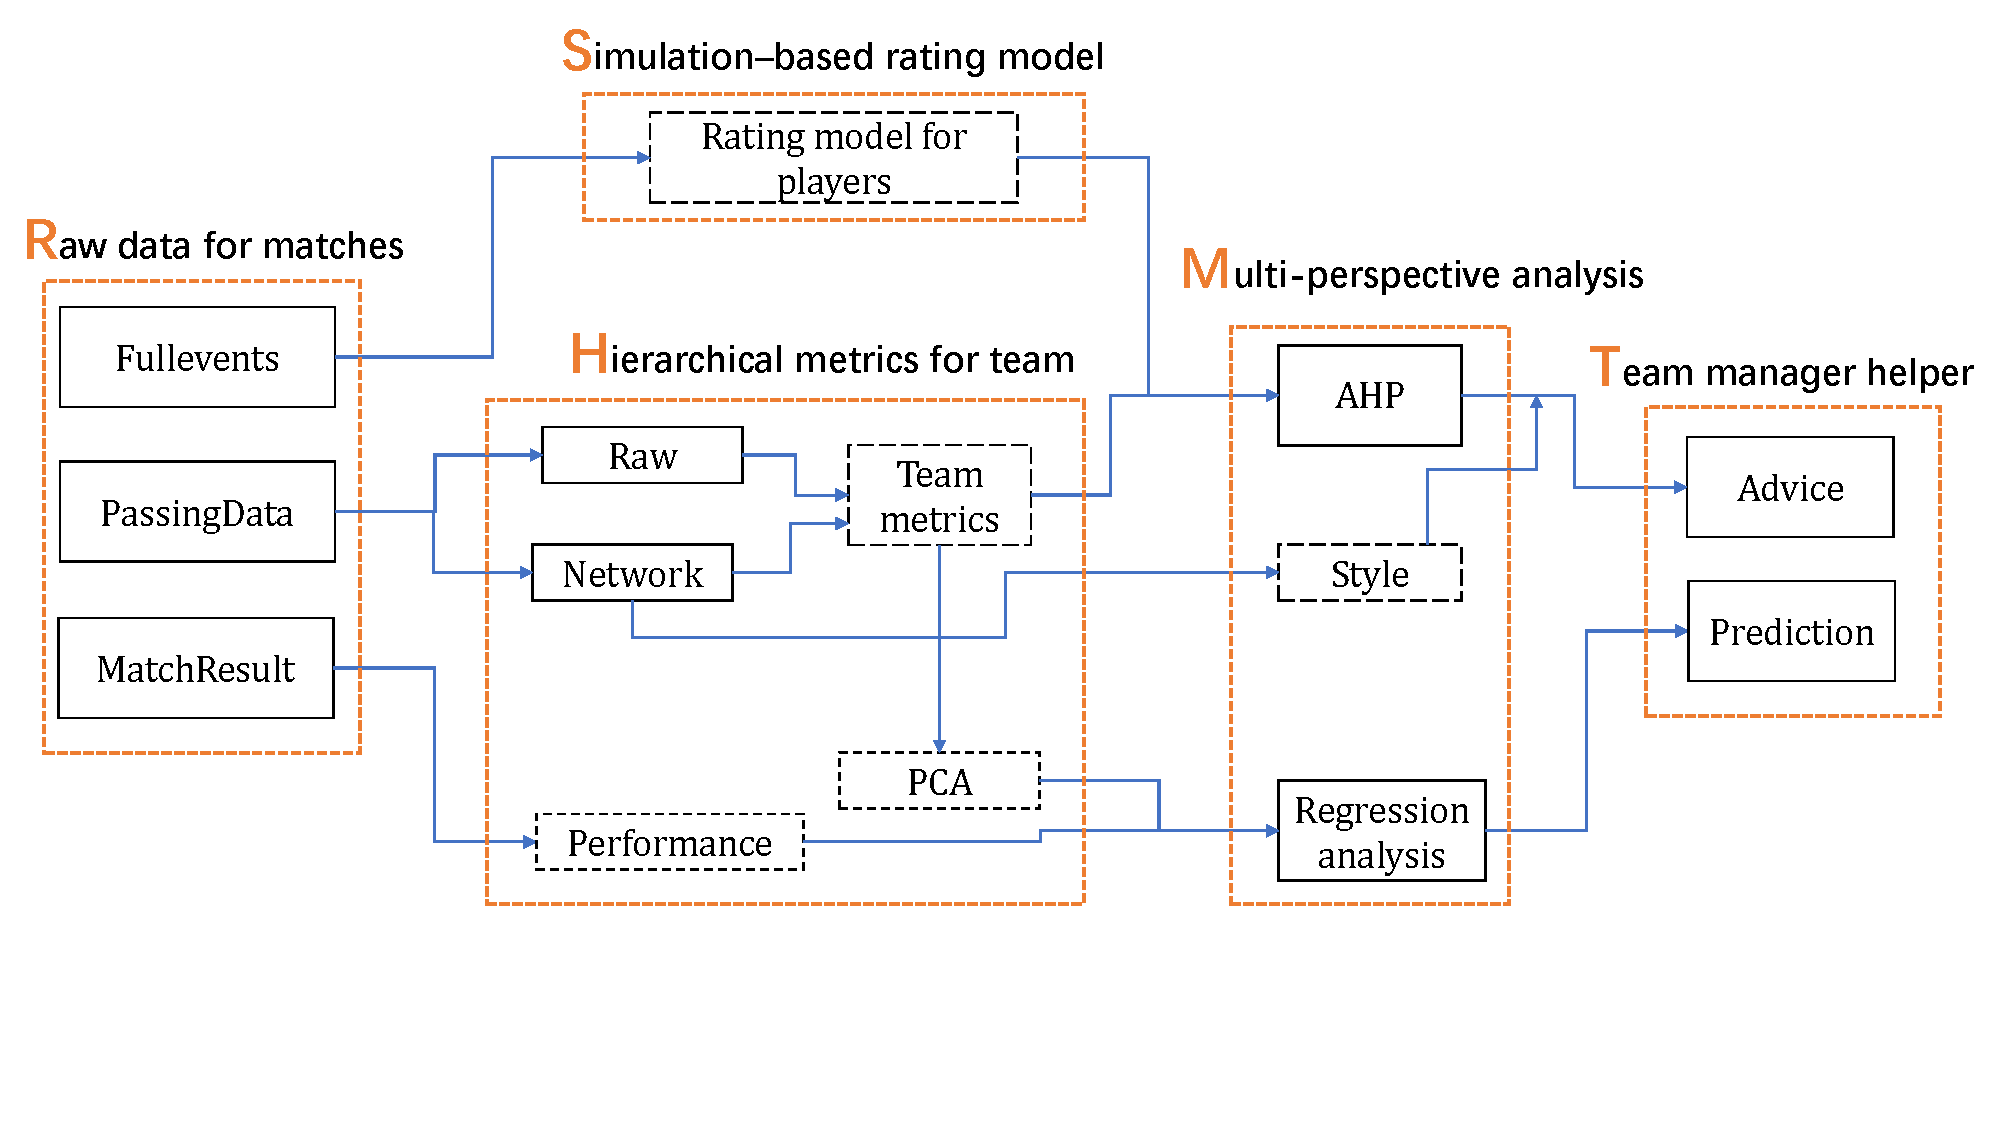
\includegraphics[width=0.8\textwidth]{flowchart.pdf}
	\caption{Flowchart of Our Model}
	\label{fig:ourwork}
\end{figure}

\section{Model Assumptions}
Our model makes the following assumptions:
\paragraph{Assumptions 1}
	\textit{We consider football field is of standard size and build Cartesian coordinates on it.}
	
	We assume that the left side of football field is the half field of our team. The origin of Cartesian coordinates is set at the lower left corner. The x-axis is along the touchline towards the right and the y-axis is along the end line upwards. We set the position of lower right corner and upper left corner (100,0) and (0,100) respectively.
\paragraph{Assumption 2}
	\textit{We assume that players pass the ball in a large number when calculating pagerank in 5.1.}
	
	In a match, well-trained players usually finish many times of passing so the assumption is reasonable and useful when we calculate pagerank below.
\paragraph{Assumption 3}
	\textit{Different kinds of behaviors in a game influence the expected number of shots in a linear model. The behaviors refer to passes, crosses, tackles, etc.} 
	
	The paper we cited has conducted a linear regression and received a sound result. Moreover, for professional teams, the number of all kinds of “behaviors” do not vary too much from game to game. So it is feasible for us to use a linear model to approximate the real influence in a relatively short interval.
\paragraph{Assumption 4}
	\textit{We assume that indicators of the whole team linearly influence the final performance of the team.}
	
	Our indicators used in this paper are directly connected with performance or style of players and the team. Therefore, we assume they linearly influence the performance. This assumption makes it possible and rational for our Principal Component Regression process below.
\section{Nomenclature}
	In this paper we use the nomenclature in Table \ref{tab:Nomen} to describe our model. Other symbols that are used only once will be described later.
	\renewcommand\arraystretch{2}
	\begin{table}[h]
		\centering
		\caption{Nomenclature}
		\label{tab:Nomen}
		\begin{tabular}{c c}
			\hline
			\textbf{Symbol} & \textbf{Definition}\\
			\hline
			$V$ & the set of vertexes\\
			$E$ & the set of edges\\
			$G$ & the graph of the network\\
		 	$n$ & the number of players in a team\\
		 	$a_{i, j}$ & the weight from node $i$ to node $j$\\
		 	$A_{n*n}$ & adjacency matrix of the graph $G$\\
		 	$p_{i}$ & the average position of the player $i$\\
		 	F, D, M, G & forward, defense, midfield, goalkeeper (respectively)\\
		 	$\mu$ & the average of passing times\\
		 	$M$ & the centroid of the team\\
		 	$d_{i ,j}$ & geodesic distance given by the length of the shortest path connecting the nodes $i$ and $j$\\
		 	$l_{i, j}$ & the reciprocal of $a_{i, j}$ (if $a_{i, j} \neq 0$)\\
		 	$C$ & the closeness centrality of a team\\
		 	$C_B (i)$ & betweenness centrality of player $i$\\
		 	$c_i$ & clustering coefficient of player $i$\\
		 	$x_i$ & pagerank score of player $i$\\
		 	$P_{i, j}$ & the shortest path from player $i$ to player $j$\\
		 	$|f|_m$ & the maximum flow of the network\\
		 	$N_e$ & edge connectivity of the network\\
		 	$W_1$, $W_2$, \ldots, $W_7$ & normalized eigenvectors of AHP\\ 
		 	$W$ & the weight vector of indicators\\
			\hline
		\end{tabular}
	\end{table}

\section{Modeling of Passing Network and Analysis}

\subsection{Our Data}
We have got the data of some football team. The data consists of three part: full events, matches, and passing events, including all 38 games the Huskies team played against their 19 opponents (they played each opposing team twice). Overall, the data covers 23,429 passes between 366 players (30 Huskies players, and 336 players from opposing teams), and 59,271 game events.

\newcommand{\tabincell}[2]{\begin{tabular}{@{}#1@{}}#2\end{tabular}}
%\begin{table}
%	\centering
%	\caption{Full Events}
%	\label{tab:full_event}
%	\begin{tabular}{|c|c|c|c|c|c|}
%		\hline
%		Match ID	&Team ID&	OriginPlayer ID&
%		Destination Player ID& Match Period	& Event Time\\
%		\hline
%		1&	Huskies&	Huskies G1	& &1H	&31.174681\\
%		\hline
%		1&	Opponent1&	Opponent1 D1&	&1H	&33.730326\\
%		\hline
%		1&	Huskies	&Huskies F1&		&1H	&33.812965\\
%		\hline
%		1&	Opponent1&	Opponent1 D2&		&1H&	42.611028\\
%		\hline
%		1&	Huskies&	Huskies D1&	Huskies F1&	1H&	46.323501\\
%		\hline
%	\end{tabular}
%	\begin{tabular}{|c|c|c|c|c|c|}
%		\hline
%		Event Type	&Event Sub-Type&	Event Origin x&	Event Origin y&\tabincell{c}	{Event\\ Destination x}&\tabincell{c} {Event\\	Destination y}\\
%		\hline
%		Free Kick&	Goal kick&	0&	0	&66	&89\\
%		\hline
%		Duel&	Air duel&	34&	11&	22&	0\\
%		\hline
%		Duel&	Air duel&	66&	89&	78&	100\\
%		\hline
%		Free Kick&	Throw in&	22&	0&	66&	3\\
%		\hline
%		Pass&	Head pass&	34&	97&	59&	95\\
%		\hline
%	\end{tabular}
%\end{table}
%
%\begin{table}
%	\centering
%	\caption{Matches}
%	\label{tab:matches}
%	\begin{tabular}{|c|c|c|c|c|c|c|}
%		\hline
%		MatchID	&OpponentID	&Outcome&	OwnScore&	OpponentScore&	Side&	CoachID\\
%		\hline
%		1&	Opponent1&	win	&1	&0&	home&	Coach1\\
%		\hline
%		2&	Opponent2&	tie	&1	&1&	away&	Coach1\\
%		\hline
%		3&	Opponent3&	loss&	0&	2&	away&	Coach1\\
%		\hline
%		4&	Opponent4&	loss&	0&	3&	home&	Coach1\\
%		\hline
%		5&	Opponent5&	loss&	0&	4&	away&	Coach1\\
%		\hline		
%	\end{tabular}
%\end{table}
%
%\begin{table}
%	\centering
%	\caption{Passing Events}
%	\label{tab:pass}
%	\begin{tabular}{|c|c|c|c|c|}
%		\hline
%		Match ID	&Team ID&	Origin Player ID&	Destination Player ID&	Match Period\\
%		\hline
%		1&	Huskies&	Huskies D1&	Huskies F1&	1H\\
%		\hline
%		1&	Huskies	&Huskies M1&	Huskies F2&	1H\\
%		\hline
%		1&	Opponent1&	Opponent1 D2&	Opponent1 G1&	1H\\
%		\hline
%		1&	Opponent1&	Opponent1 G1&	Opponent1 F1&	1H\\
%		\hline
%		1&	Huskies	&Huskies M2	&Huskies M3&	1H\\
%		\hline
%	\end{tabular}
%	\begin{tabular}{|c|c|c|c|c|}
%		\hline
%		Event Sub-Type&	Event Origin x	&Event Origin y&	\tabincell{c}{Event\\Destination x}	&\tabincell{c}{Event\\ Destination y}\\
%		\hline
%		Head pass	&34&	97	&59&	95\\
%		\hline
%		Simple pass	&53	&89&	69	&91\\
%		\hline
%		Simple pass	&19	&16	&5	&50\\
%		\hline
%		Launch&	5	&50	&67	&44\\
%		\hline
%		Simple pass	&42	&55&	36&	54\\
%		\hline
%	\end{tabular}
%\end{table}
%Table \ref{tab:full_event}, \ref{tab:matches}, and \ref{tab:pass} show part of the data. Table \ref{tab:full_event} shows the basic events in the matches such as ``Duel'' and ``Pass'' and their detailed information. Table \ref{tab:matches} shows the information about matches such as scores and coaches. Table \ref{tab:pass} shows the passing events happened in matches and we can roughly figure out the running route of the ball.
%We can analyze players' behavior and cooperation based on these data.

\subsection{Model of Passing Network}
To discover the cooperation and other patterns of the football team, we build a network model to identify the locations of players and the passing events between two players.

Consider each player as a vertex and the passing routes between players as edges, then we will get a graph:
\begin{equation}\label{eq:graph}
G = \left[V, E\right]
\end{equation}
where:
\begin{itemize}
	\item $V$ represents the set of vertexes;
	\item $E$ represents the set of edges;
	\item $G$ represents a graph.
\end{itemize}

Weight of each edge is defined as the time of passing from the source of the edge to its destination. The graph $G$ is an directed graph. As common, the in-degree of each node represents the number of passes made towards this player, while the out-degree of each node represents the number of passes made from this player. We use $a_{i, j}$ to represents the weight of the edge from node $i$ to node $j$. In this way, we get a adjacency matrix of graph $G$, we use the adjacency map $A_{n \times n}$ to represent it.
%\begin{equation}\label{eq:ad_matrix}
%A_{n*n} =
%\begin{bmatrix}
%a_{1, 1} & a_{1, 2} &\cdots &a_{1, n}\\
%a_{2, 1} & a_{2, 2} &\cdots &a_{2, n}\\
%\vdots & \vdots & \ddots & a_{n-1, n}\\
%a_{n, 1} & a_{n, 2} & \cdots & a_{n, n}\\
%\end{bmatrix}
%\end{equation}

We use $p_{i}$ to represents the average position of the player $i$ in the network. $p_{i}$ can be calculated as follows:
\begin{align}\label{eq:pos}
\text{the x coordinate of } p_{i}&=\frac{x_1 + x_2 +\dots +x_{N_{pos}}}{N_{pos}}\nonumber\\
\text{the y coordinate of } p_{i}&=\frac{y_1 + y_2 +\dots +y_{N_{pos}}}{N_{pos}}
\end{align}
where:
\begin{itemize}
	\item $x_{i}$ represents the x coordinate of the $i_{th}$ position;
	\item $y_{i}$ represents the y coordinate of the $i_{th}$ position;
	\item $N_{pos}$ represents the number of position data.
\end{itemize}

We will plot the network of the football team based on $A_{n*n}$ and $p_{i}$.

The network described above is a static one, but in real matches, the graph changes through time, which requires us to find other features of the passes. The number of triangles in a network is an important feature of the network and can help us analyze the team formation. The \textbf{triangle} in a network can be described as three nodes that are directly connected. To simplify the problem and calculate the result, we assume the graph $G$ is undirected in this part of our model, and add the weight $a_{i, j}$ and $a_{j, i}$ together as $a^{'}_{i, j}$. So the triangles we want to find is just the so-called K3 complete subgraph.~\cite{defining}

To help evaluate how well a team plays in an objective manner, we also introduce the performance of the team in the whole season:
\begin{equation}\label{eq:perform}
performance = \left(0.3 \times N_{goal-difference} + 0.7 \times points \right) \times k + 2
\end{equation}
where:
\begin{itemize}
	\item $N_{goal-difference}$ is the goal difference;
	\item $points$ is the points that the team gets in the match. If they wins, ties, and loses, they will get 3, 1, and 0 points respectively;
	\item $k$ is a parameter. $k$ of home team is 0.9 and $k$ of guest team is 1.
\end{itemize}

\subsection{Analysis of Passing Network and its Features}
\paragraph{Heatmap of the Ball}
First of all , in order to make a rough view on the playing pattern of Huskies, we plot heatmaps of passing events in Figure \ref{fig:heatmap}. The home team always kicks the ball from left to right in these figures. From th figure, we find that the starting positions of our ball are mostly distributed in the backfield and midfield while the ending positions of our ball are more closed to the opponent's goal. However, after comparing carefully between the heatmap of Huskies team and the opponents, we find that passes performed by Huskies are more clustered in the left part of the field, which may indicate the difficulty the team encounters in delivering the football forward.

\begin{figure}[h]
	\centering
	\begin{subfigure}[b]{0.23\textwidth}
		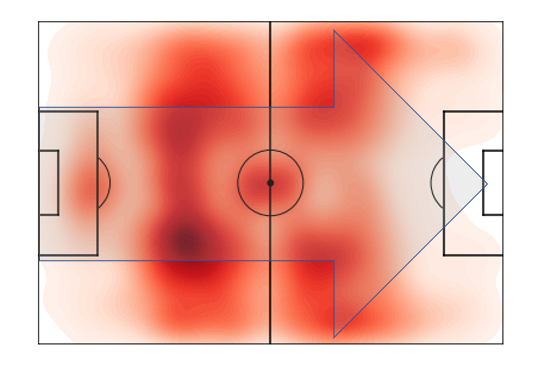
\includegraphics[width=\textwidth]{heatmap_start.png}
		\caption{Heatmap of Starting Position of Our Ball}
	\end{subfigure}
	\begin{subfigure}[b]{0.23\textwidth}
		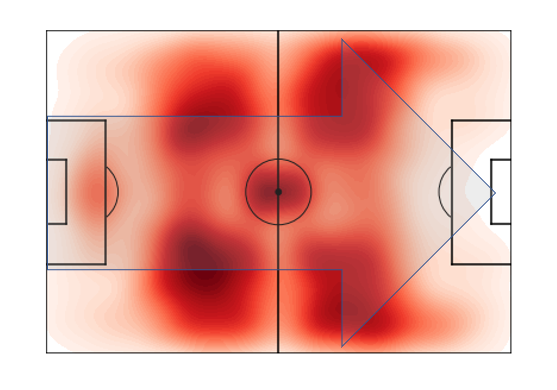
\includegraphics[width=\textwidth]{heatmap_start_opponent.png}
		\caption{Heatmap of Starting Position of Rival Ball}
	\end{subfigure}
	\begin{subfigure}[b]{0.23\textwidth}
		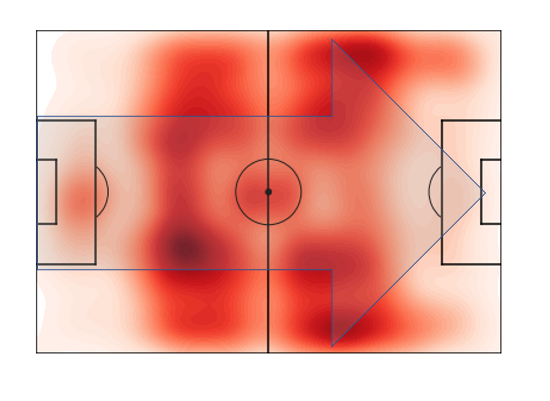
\includegraphics[width=\textwidth]{heatmap_end.png}
		\caption{Heatmap of Ending Position of Our Ball}
	\end{subfigure}
	\begin{subfigure}[b]{0.23\textwidth}
		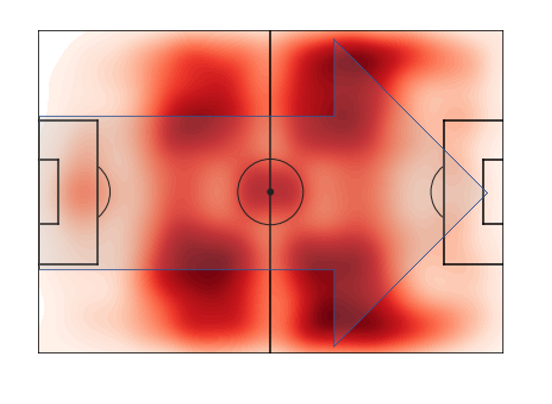
\includegraphics[width=\textwidth]{heatmap_end_opponent.png}
		\caption{Heatmap of Ending Position of Rival Ball}
	\end{subfigure}
	\caption{Heatmap of the Ball}
	\label{fig:heatmap}
\end{figure}


\begin{figure}[h]
	\centering
	\begin{subfigure}[b]{0.4\textwidth}
		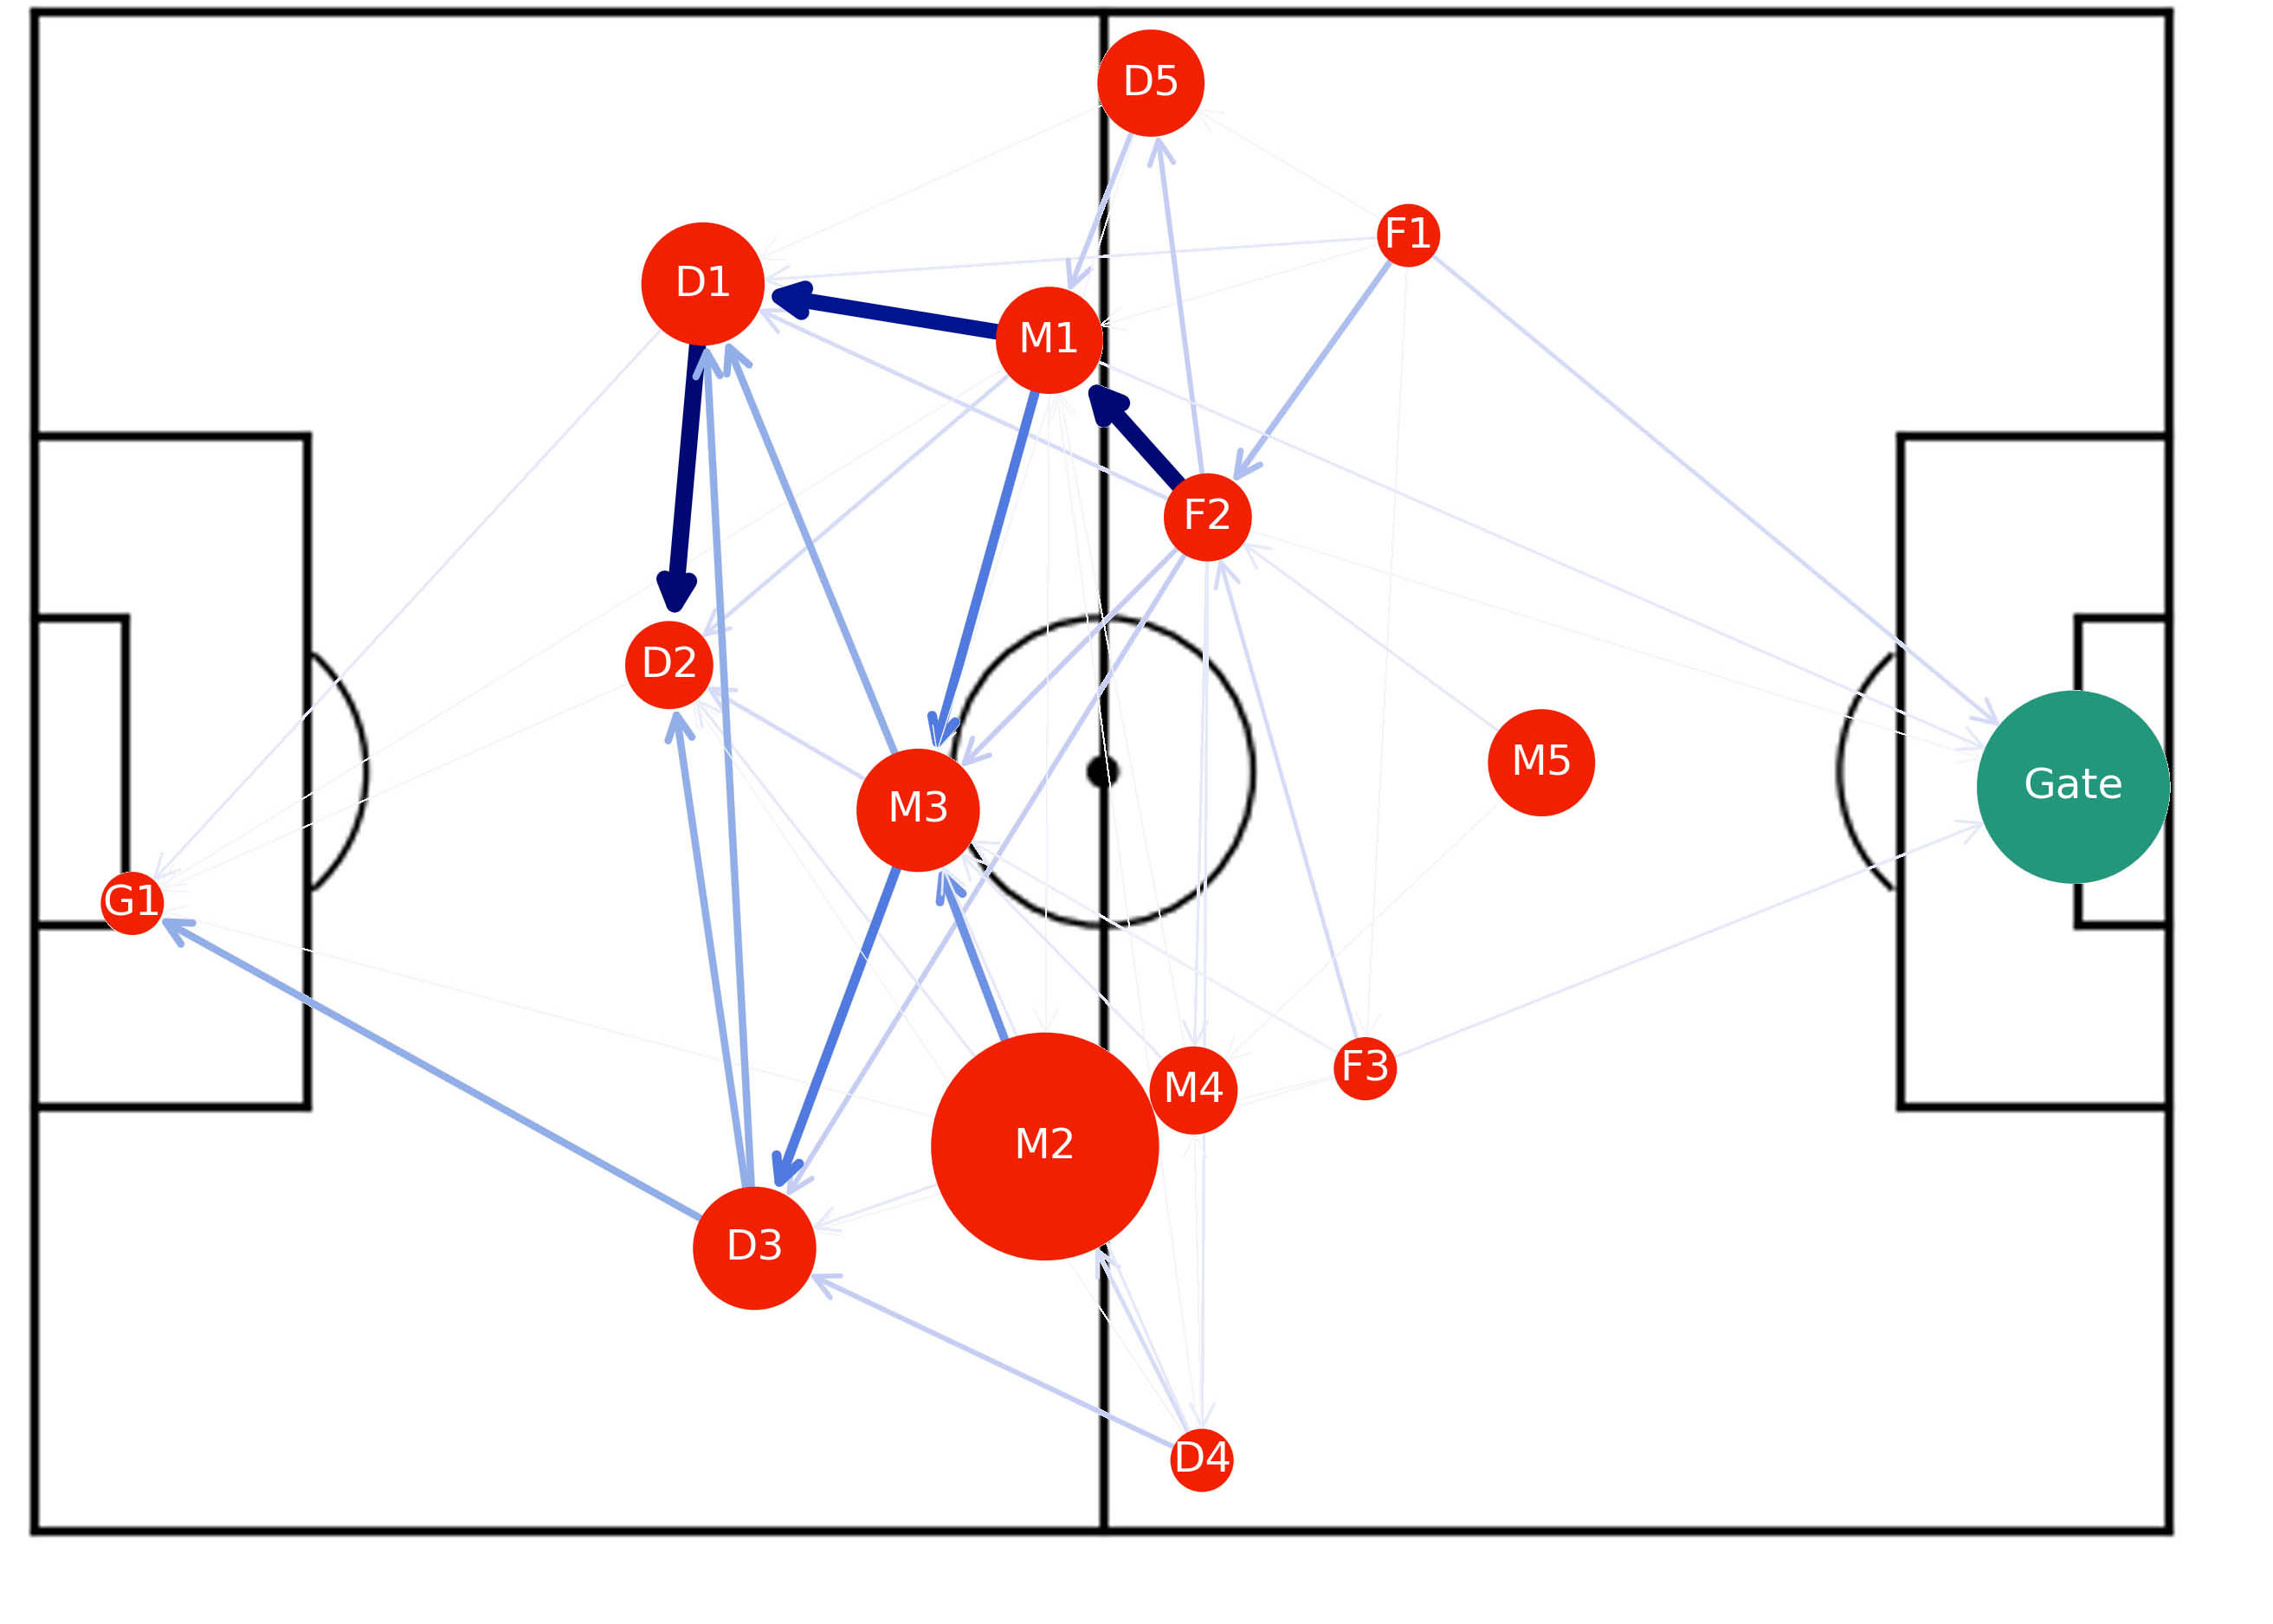
\includegraphics[width=\textwidth]{nn_mathid_dir_forward1.jpg}
		\caption{}
	\end{subfigure}
	\begin{subfigure}[b]{0.4\textwidth}
		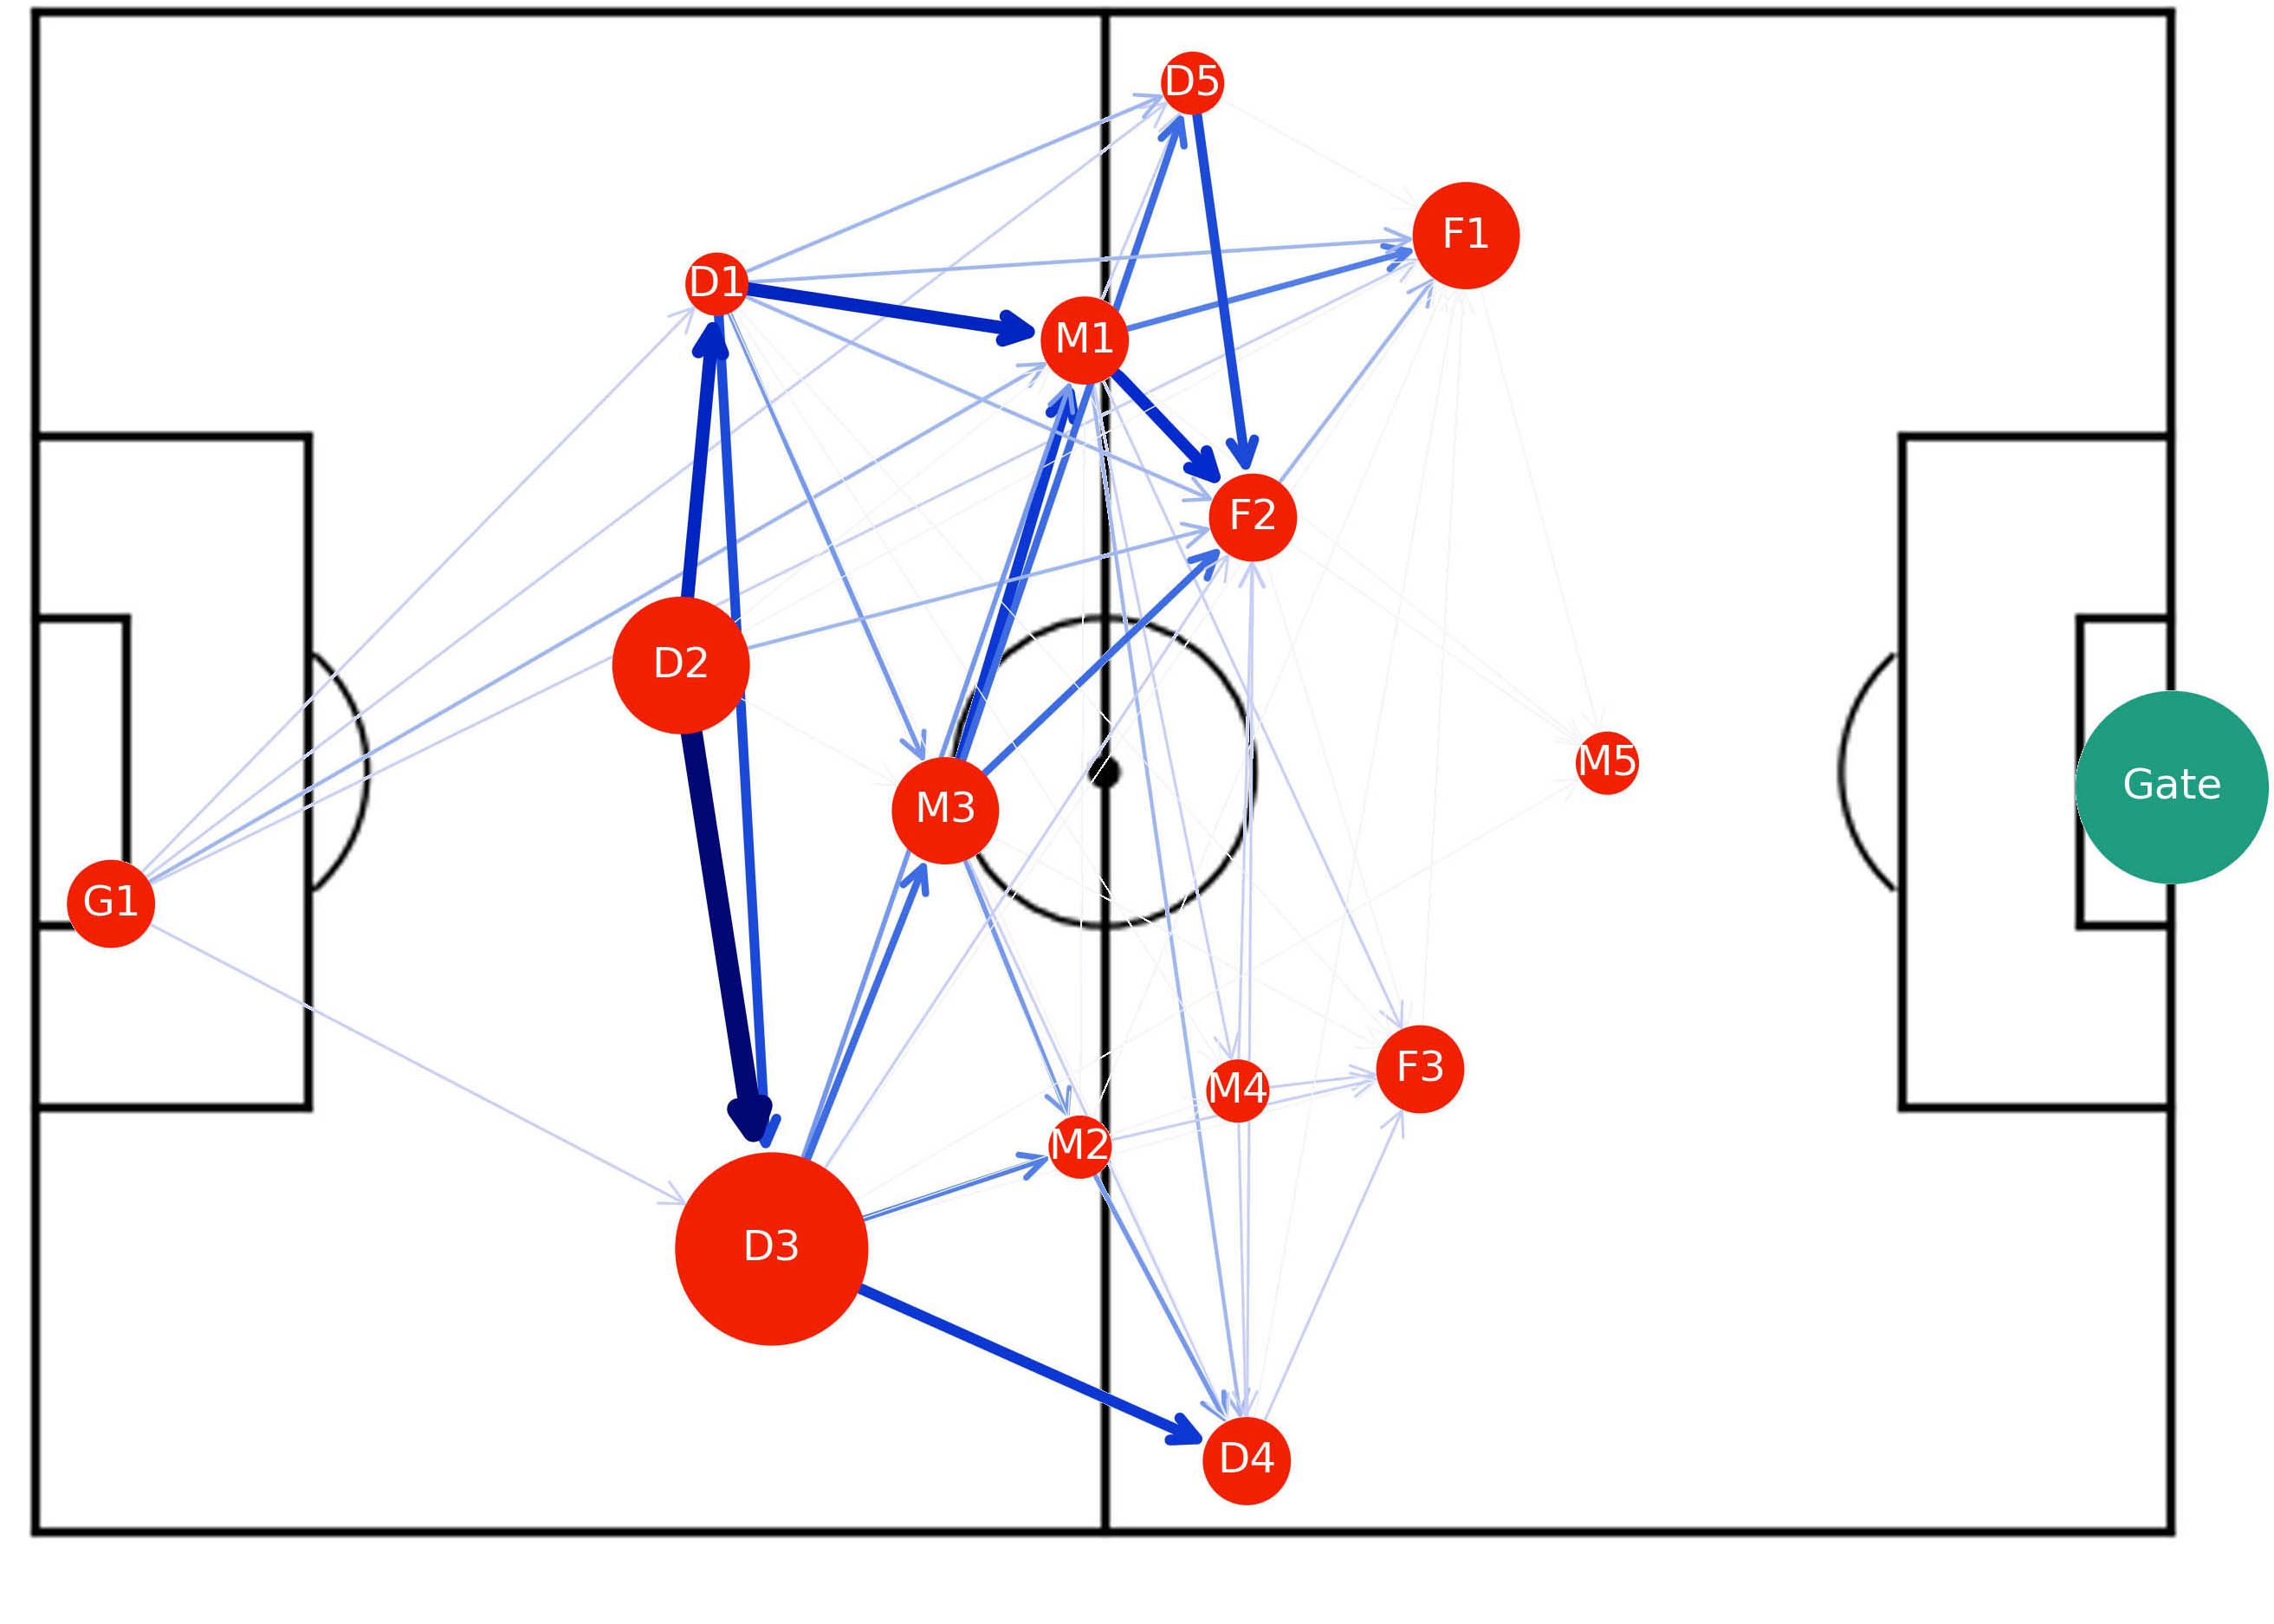
\includegraphics[width=\textwidth]{nn_mathid_dir_backward1.jpg}
		\caption{}
	\end{subfigure}
%	\begin{subfigure}[b]{0.4\textwidth}
%		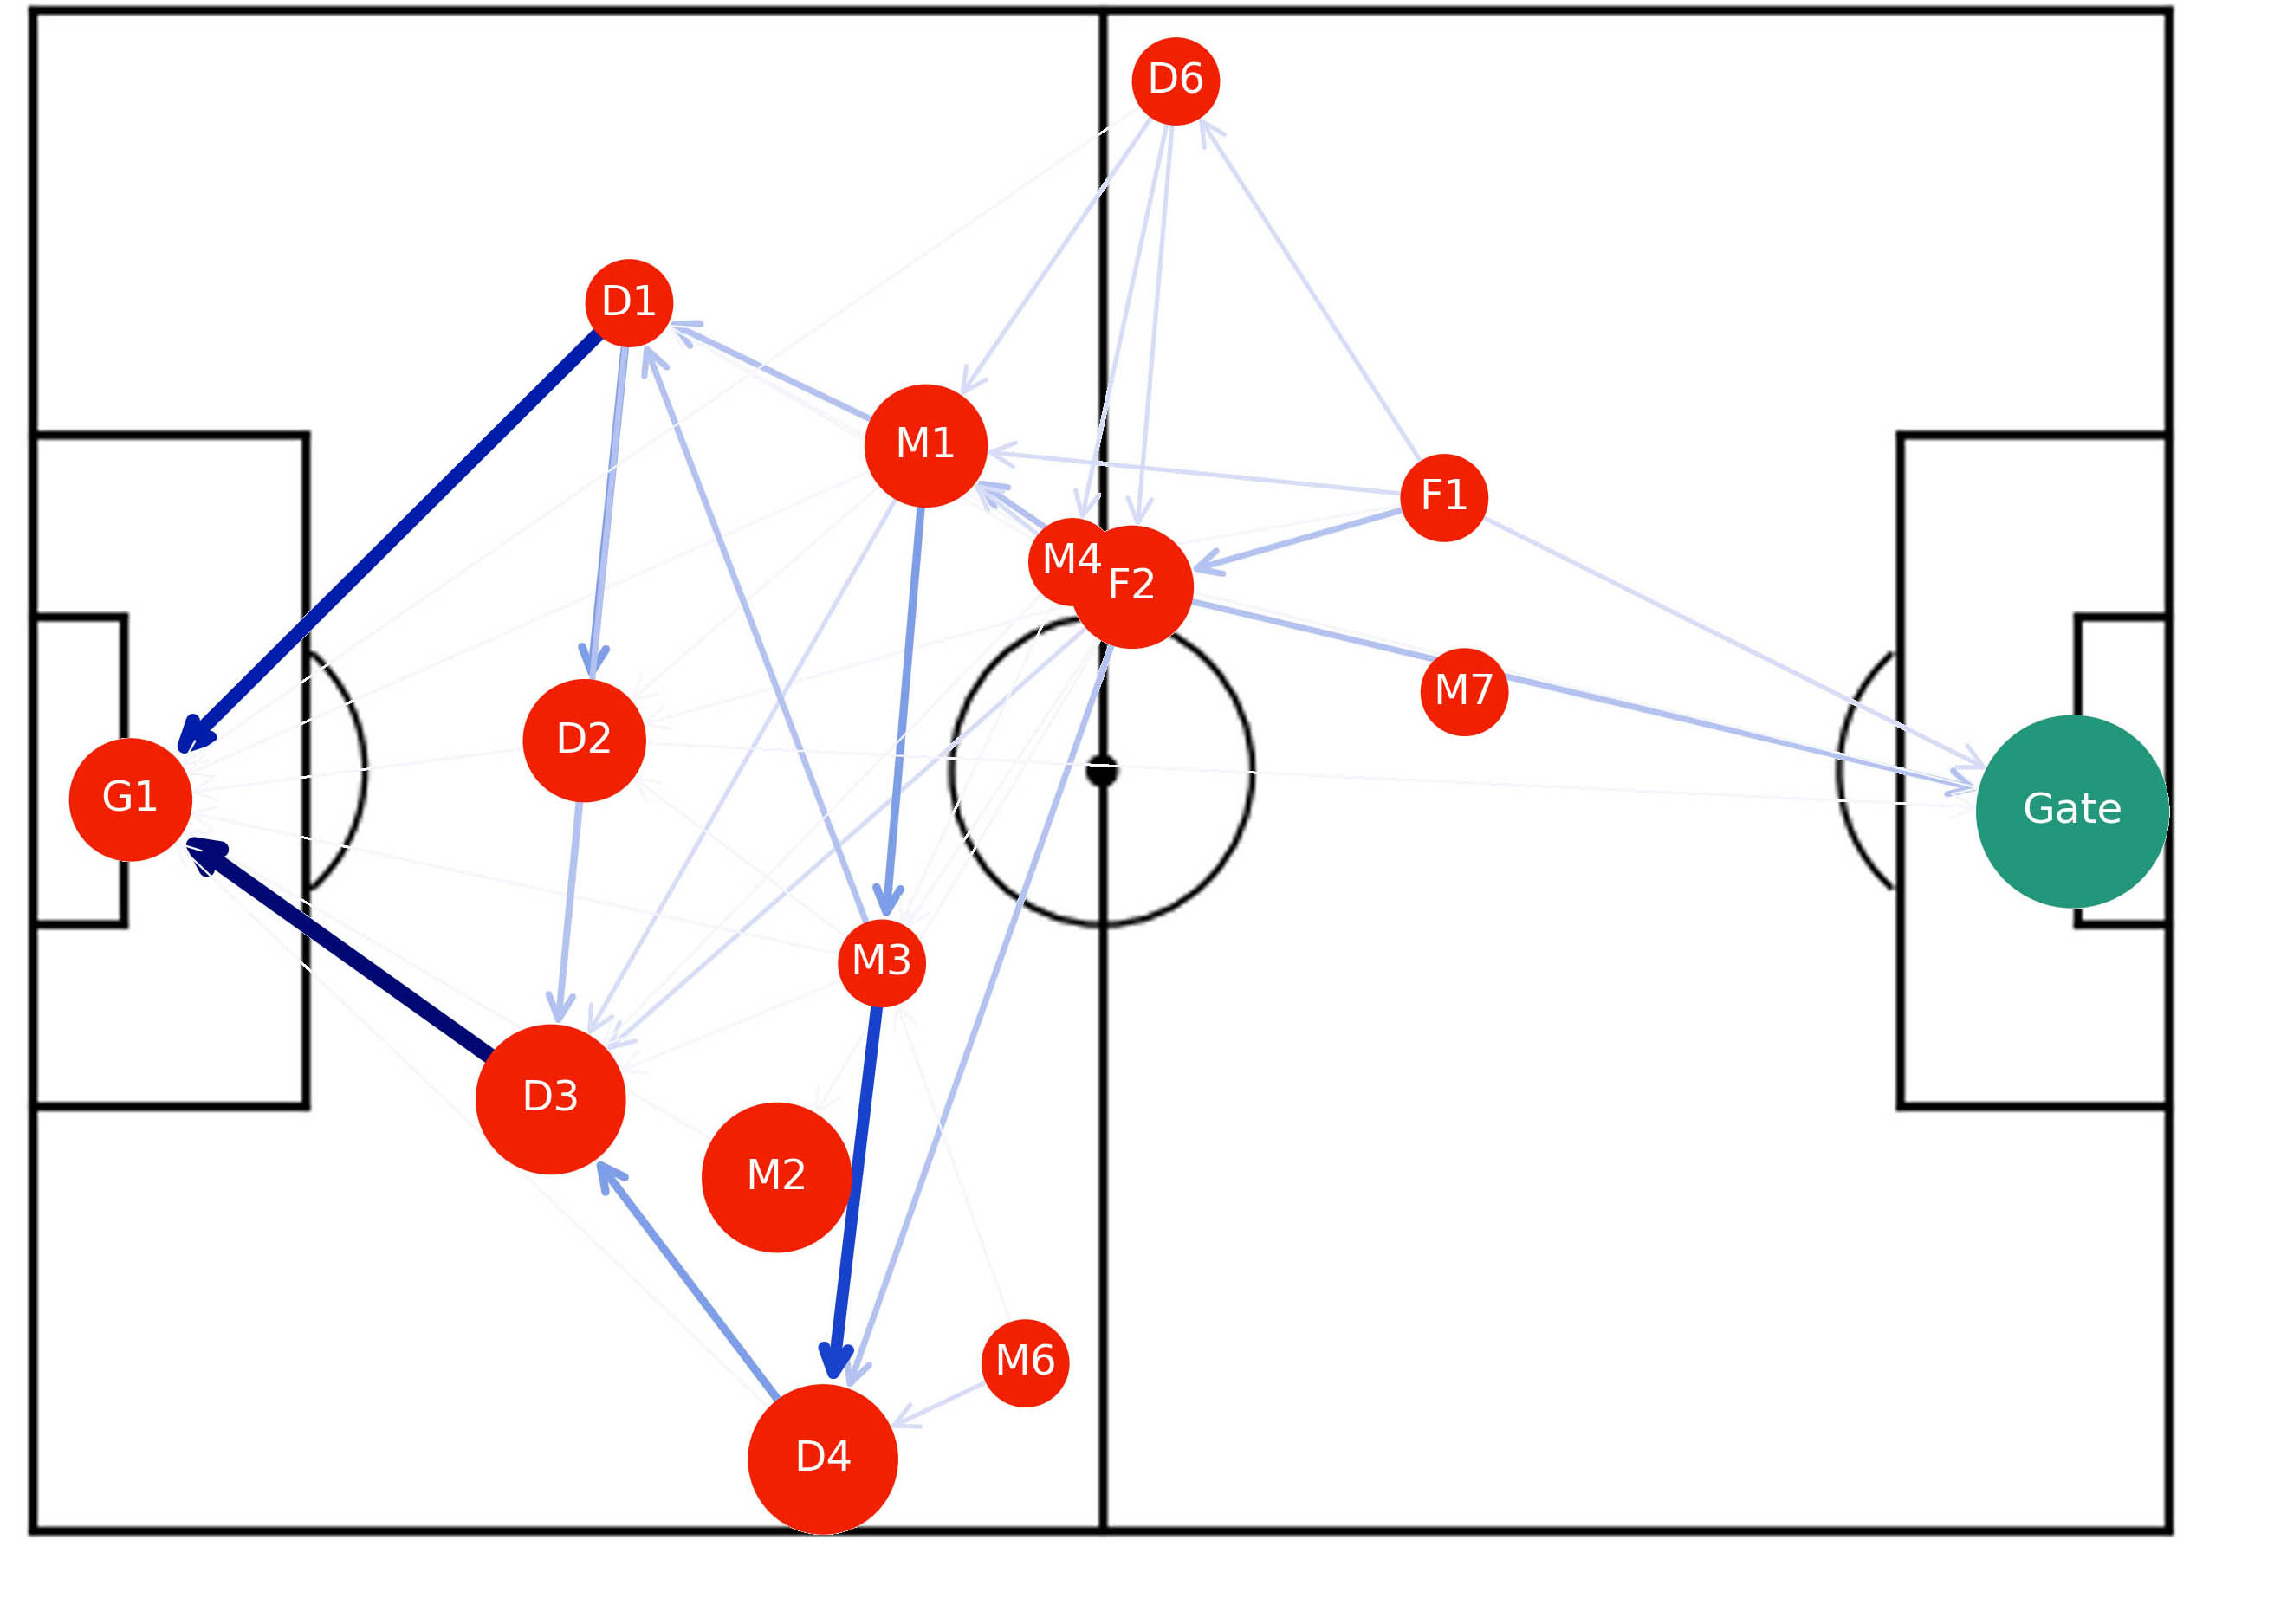
\includegraphics[width=\textwidth]{nn_mathid_dir_forward2.jpg}
%		\caption{}
%	\end{subfigure}
%	\begin{subfigure}[b]{0.4\textwidth}
%		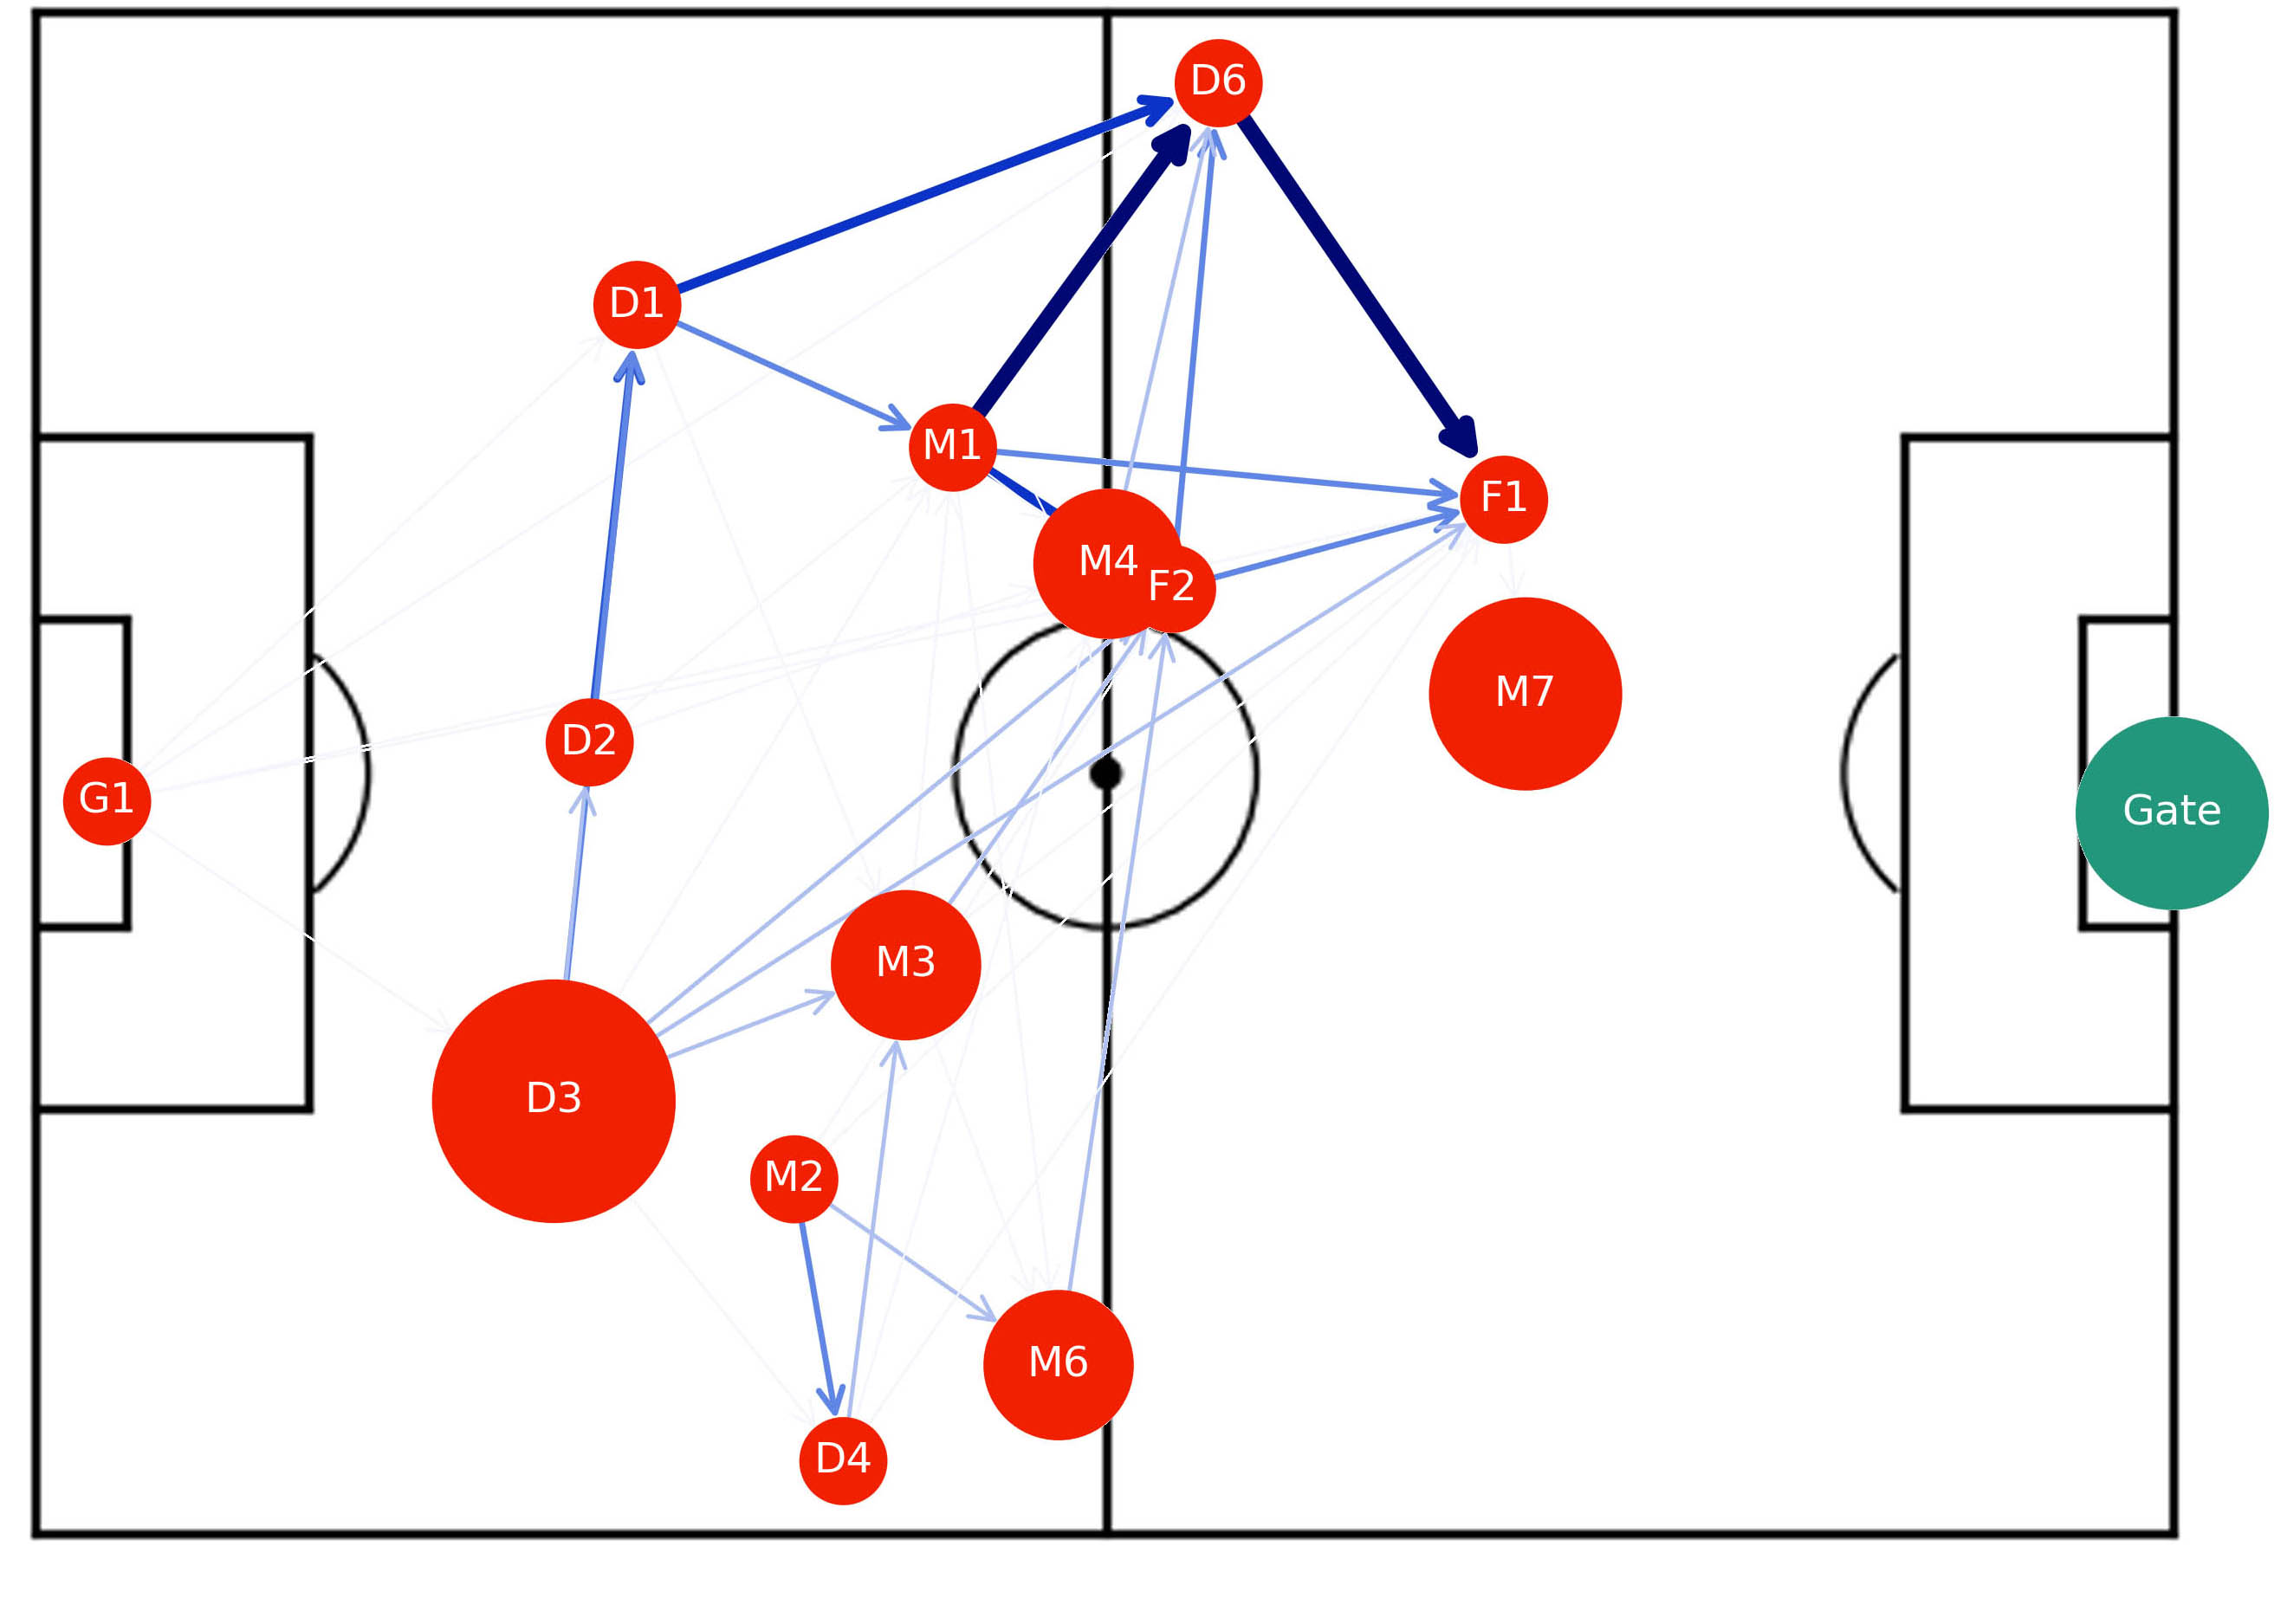
\includegraphics[width=\textwidth]{nn_mathid_dir_backward2.jpg}
%		\caption{}
%	\end{subfigure}
	\begin{subfigure}[b]{0.4\textwidth}
		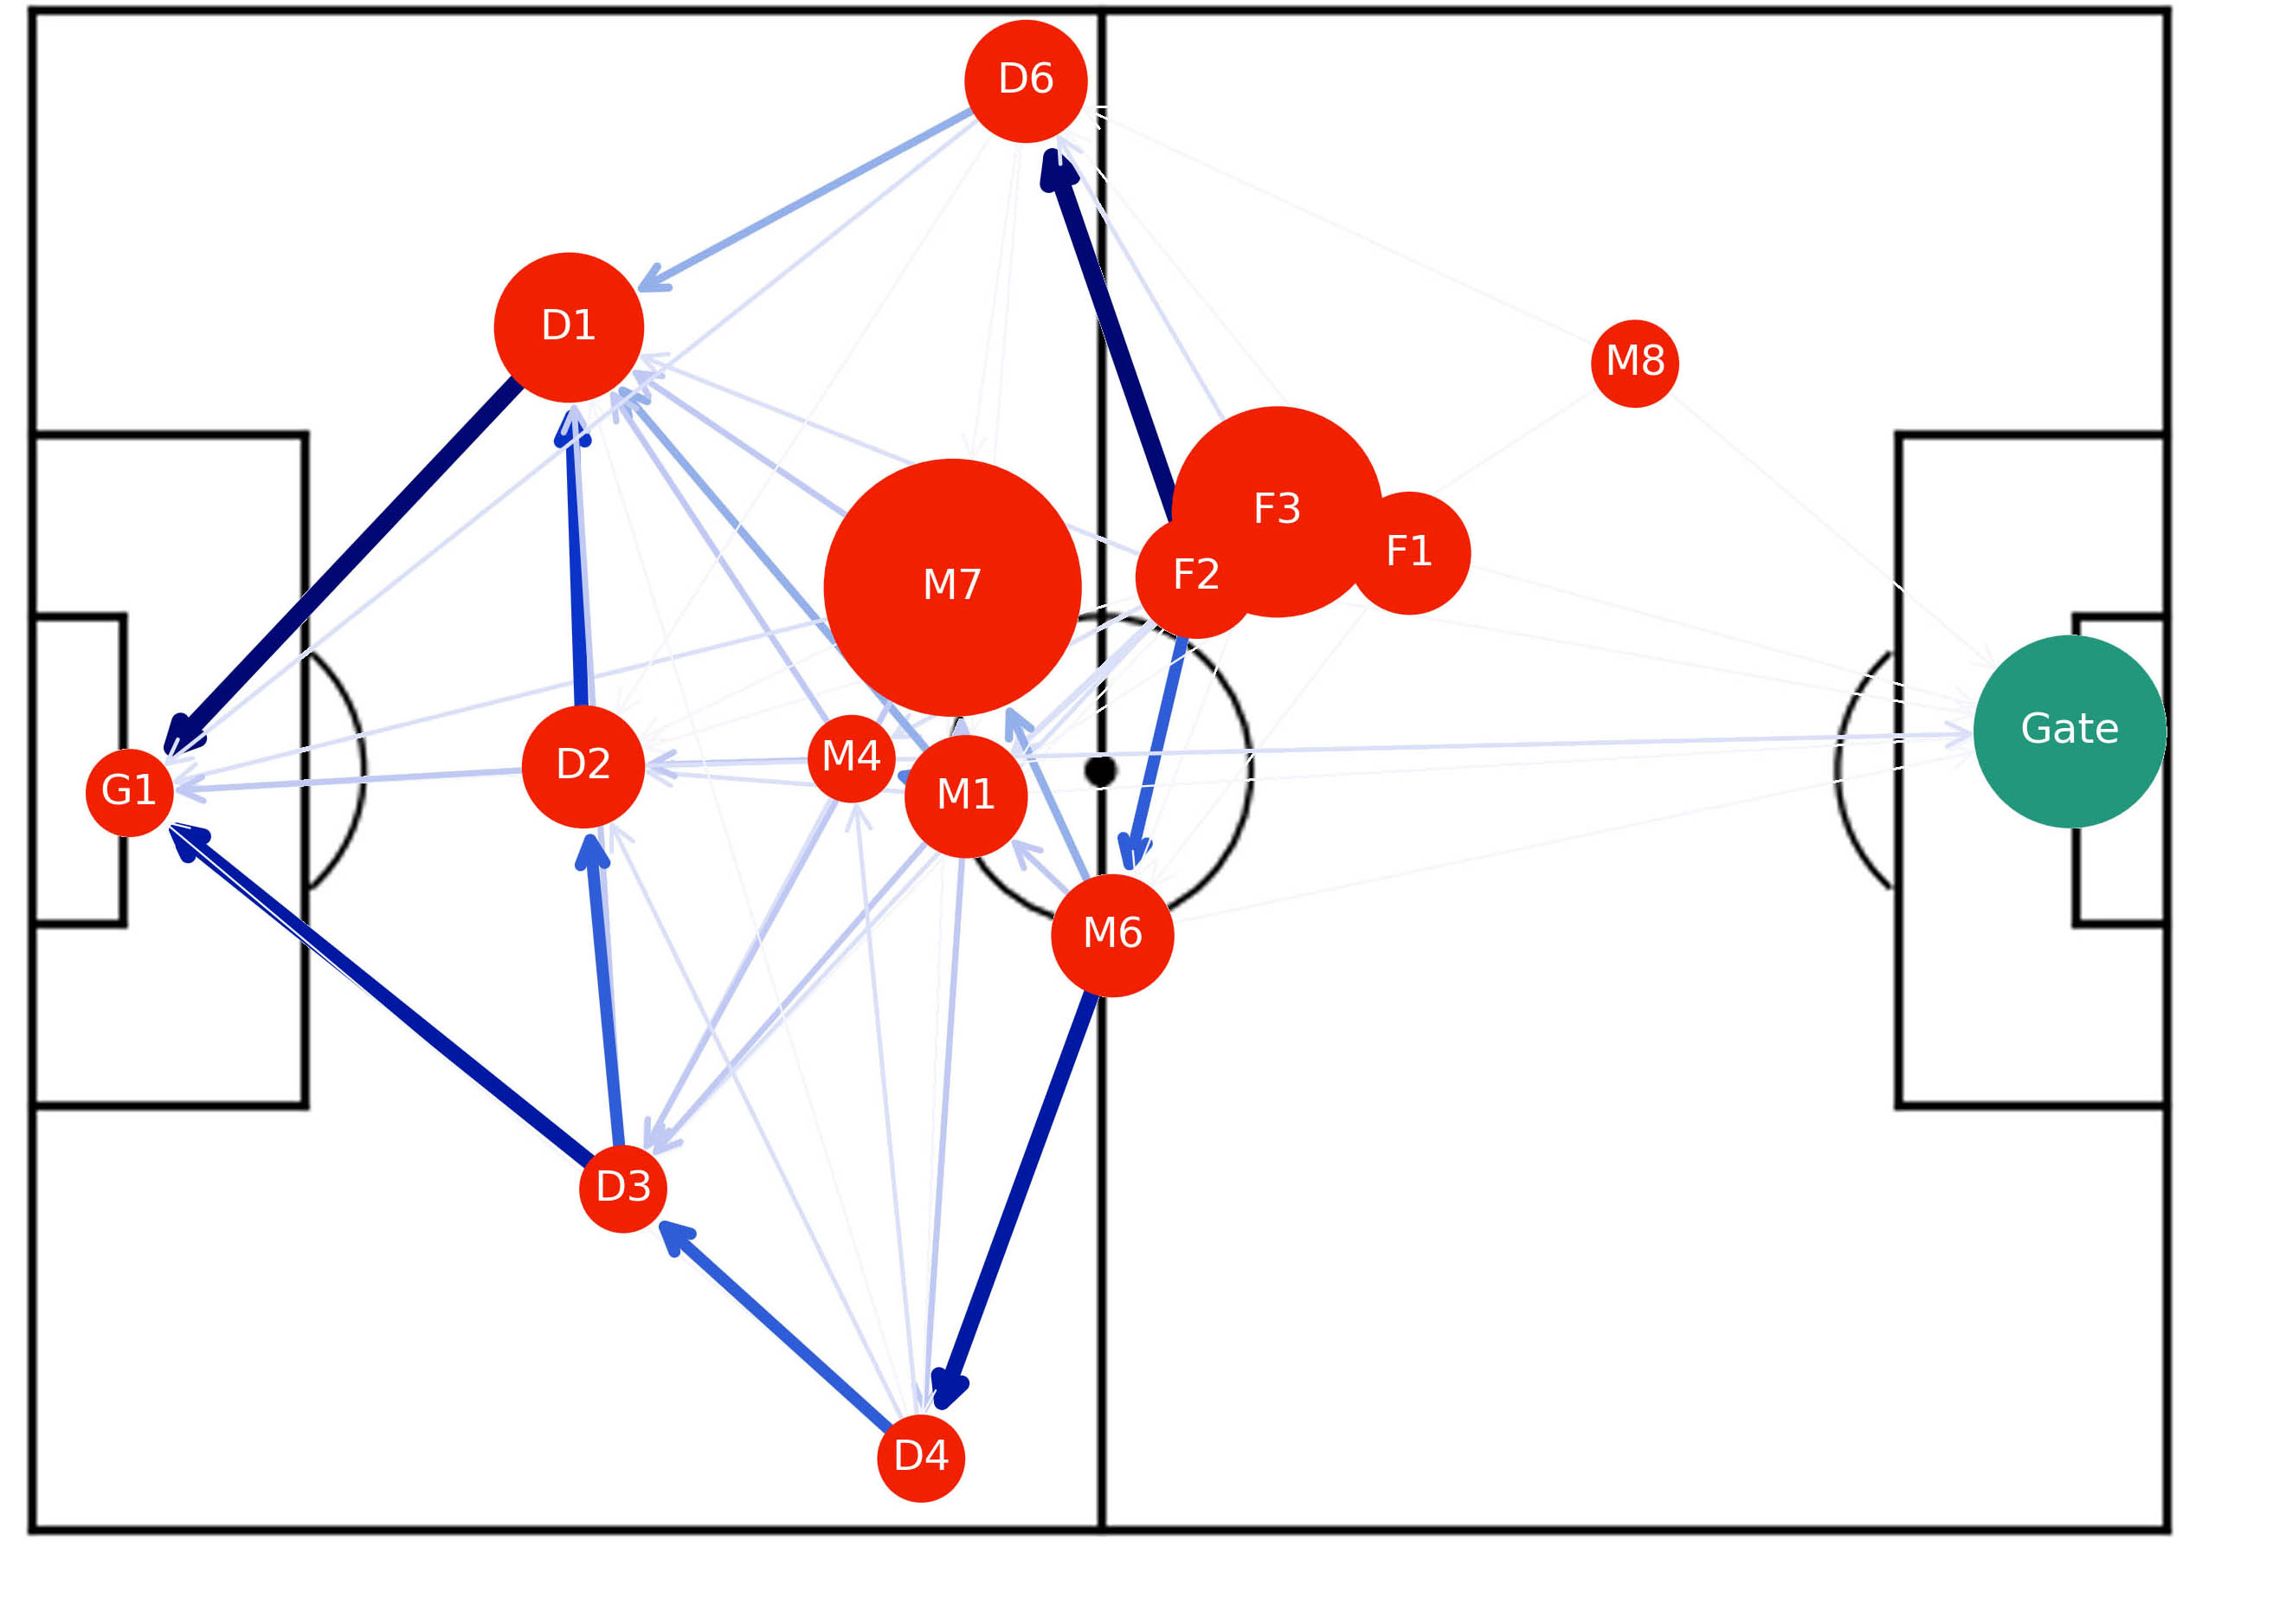
\includegraphics[width=\textwidth]{nn_mathid_dir_forward3.jpg}
		\caption{}
	\end{subfigure}
	\begin{subfigure}[b]{0.4\textwidth}
		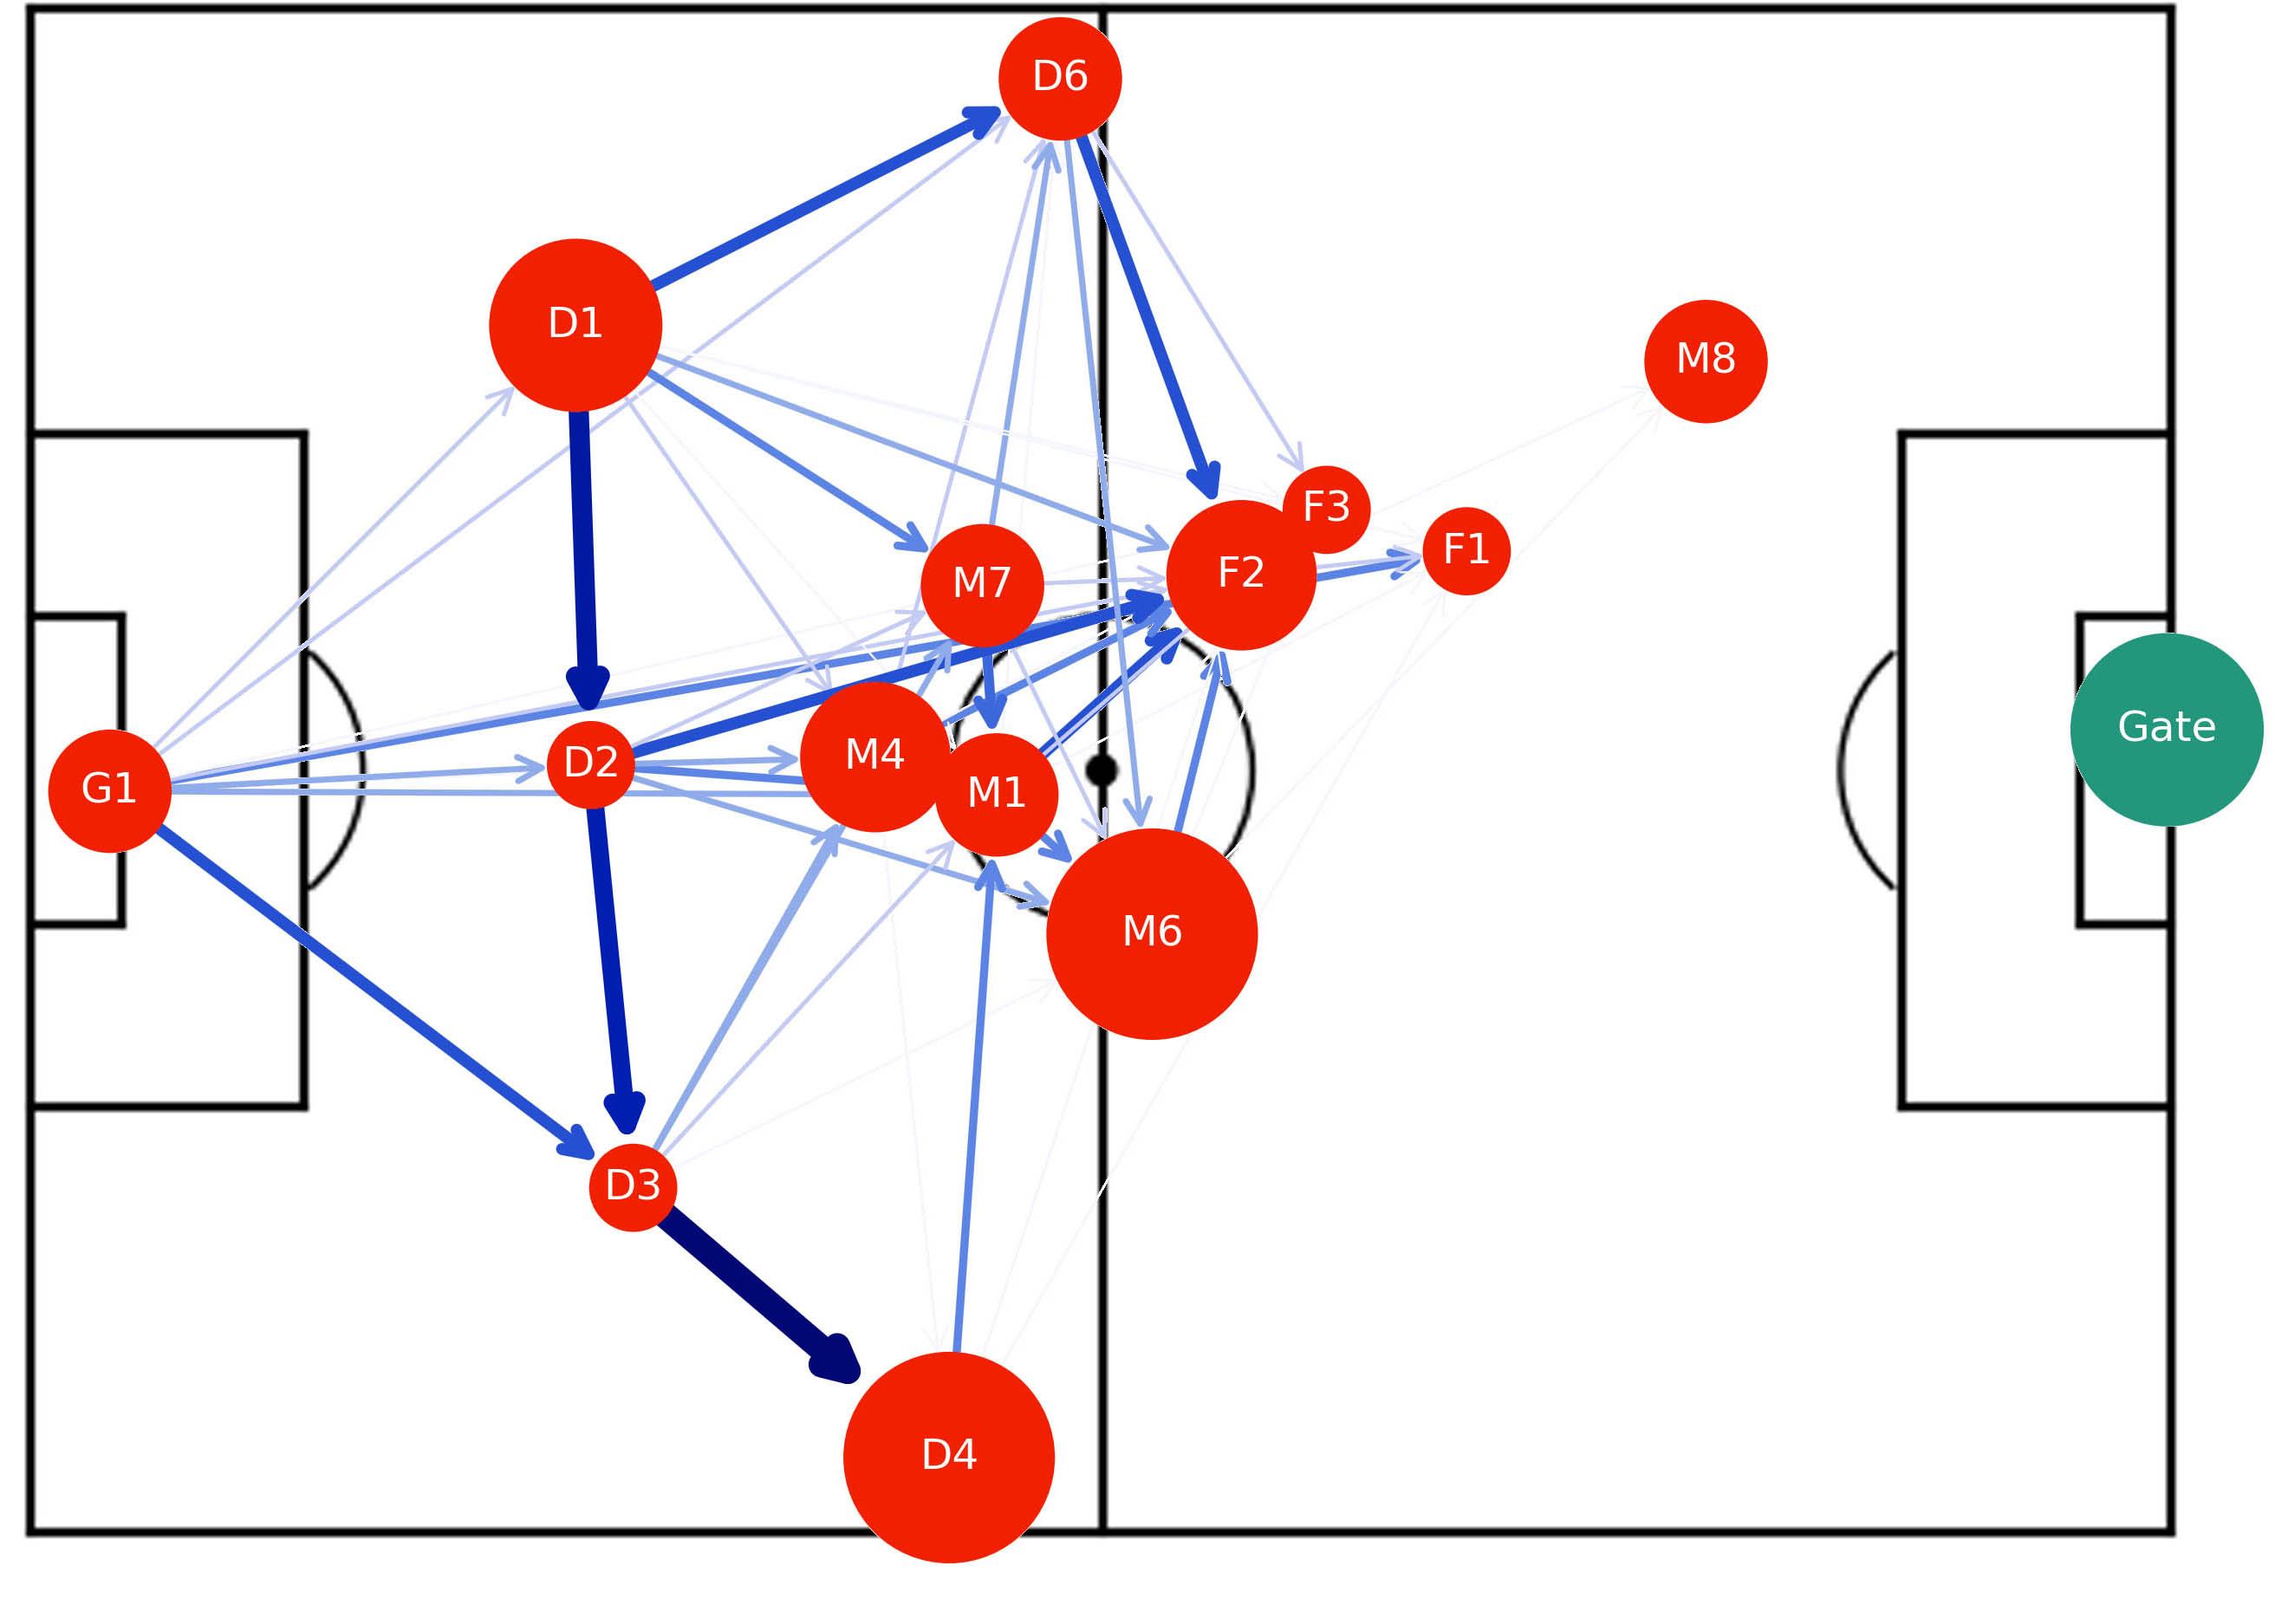
\includegraphics[width=\textwidth]{nn_mathid_dir_backward3.jpg}
		\caption{}
	\end{subfigure}
	\caption{Network of the Huskies Team (a) is the backward passing network of match 1; (b) is the forward passing network of match 1; %(c) is the backward passing network of match 2; (d) is the forward passing network of match 2; 
(c) is the backward passing network of match 3; (d) is the forward passing network of match 3.}
	\label{fig:network}
\end{figure}

\paragraph{General Analysis of Network}
After a brief look at the Huskies' passing pattern, we use the Equation \ref{eq:graph} and \ref{eq:pos} to calculate the positions of nodes and the weights of edges. Too solve the problem of edge overlap, we \textbf{divide the original graph into two subgraphs} and plot team network and the background is a standard football field. We plot the forward and backward passing network of 2 matches whose ID are 1 and 3 and the Huskies Team won and lost the match respectively.

As we can see in Figure \ref{fig:network}, each network has several edges that are connected with each other closely, which indicates that this football team has well-trained passing routes. Compared to Figure \ref{fig:network} (a) and (b), in Figure \ref{fig:network} (e) and (f), the backward passing network is more closely connected than the forward passing network. We could conclude from the figure that the team is more defensive in the match that it loses, which may imply that the team needs to play more aggressively.~\cite{gursakal}

\begin{figure}[h]
	\centering
	\begin{subfigure}[b]{0.46\textwidth}
		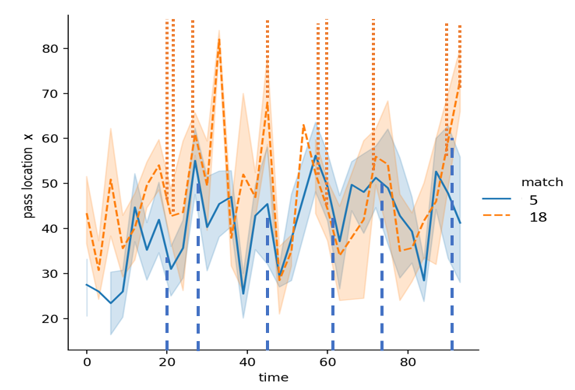
\includegraphics[width=\textwidth]{passlocation.PNG}
		\caption{X-axis coordinate of passes through time}
	\end{subfigure}
	\begin{subfigure}[b]{0.46\textwidth}
		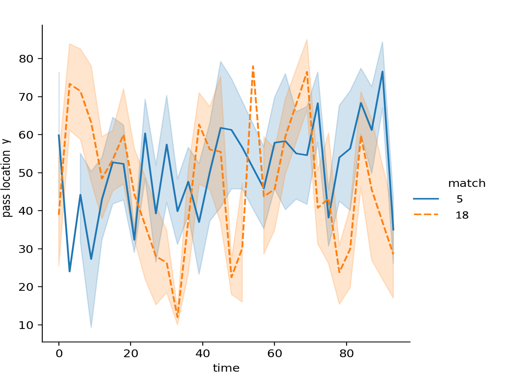
\includegraphics[width=\textwidth]{passfig2.png}
		\caption{Y-axis coordinate of passes through time}
	\end{subfigure}
	\caption{Analysis of the spatial distribution of passes through time}
	\label{fig:pass_distribution}
\end{figure}
In Figure \ref{fig:pass_distribution}, we visualize the spatial distribution of passes during different time of day. The lines in subfigure[a] show the variation in the x-axis coordinate of passes(the direction from the home goal to the away goal) in match 5 (Huskies lost by 4:0) and match 18 (Huskies won by 3:1). The dotted lines above and below the shade refers to a shot. We can conclude from it that the shots often occur when the team is constantly sending the ball forward. And the subfigure [b] shows the variation in the y-axis (across the field) coordinate of passes. We note that in the game that Huskies won, they try more long passes across the field. In this way, they successfully mobilize opponents' defence line, and thus win more opportunities for shots. The strategy is quite wise.
\begin{figure}[h]
	\centering
	\begin{subfigure}[b]{0.47\textwidth}
		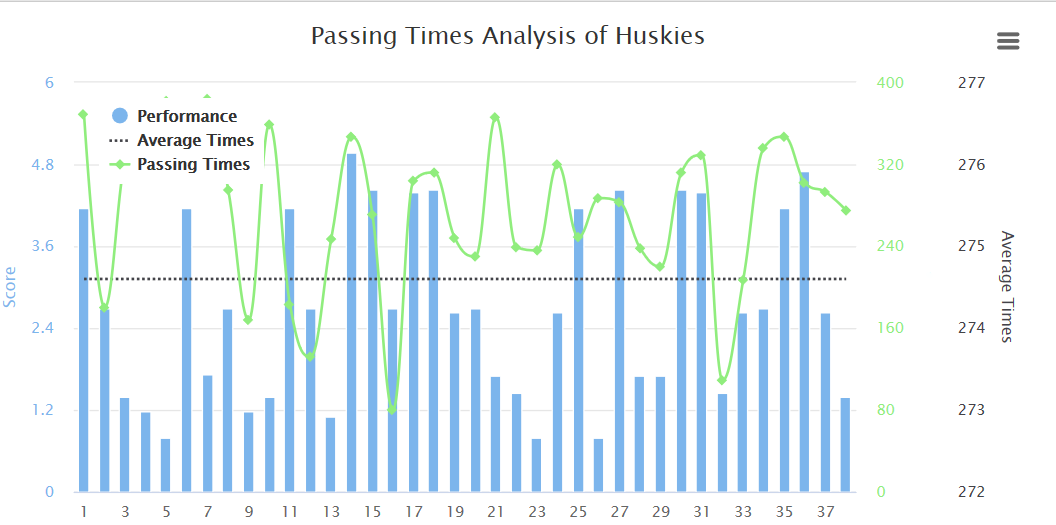
\includegraphics[width=\textwidth]{triangle_season.PNG}
		\caption{}
	\end{subfigure}
	\begin{subfigure}[b]{0.47\textwidth}
		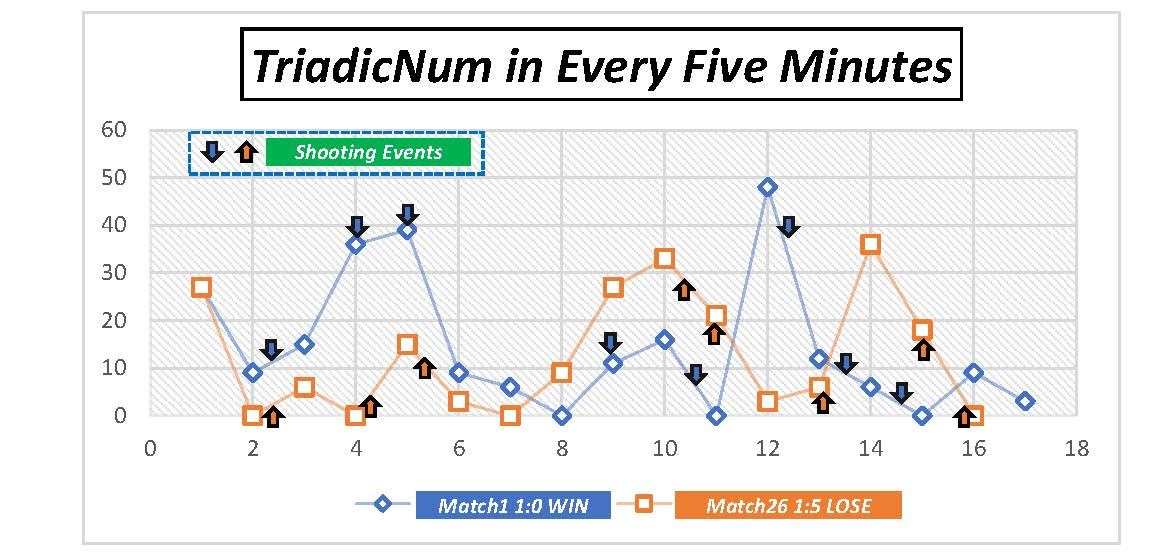
\includegraphics[width=\textwidth]{triadic.pdf}
		\caption{}
	\end{subfigure}
	
	\caption{Triangles of Some Matches and Passing Times of a Whole Season (a) shows the passing times of the whole season; (b) shows the number of triangles formed in every five minutes in two matches.}
	\label{fig:triangle}
\end{figure}
\paragraph{Triadic Analysis of Network}
Figure \ref{fig:triangle} (a) shows the performance of Huskies team in the whole season. The $performance$ is calculated by Equation \ref{eq:perform}. We discover that the $performance$ tend to be high when the number of passing times is above the average and low $performance$ usually reflects on the fewer passing times.

From Figure \ref{fig:triangle} (b) we can discover that in match 1 the team are more likely to make a shoot when the number of triangles increases. So the team is more likely to score and win the match.~\cite{common} However, in match 26, the number of triangles is fewer so the team finally lose the match. The shoots are possibly not well-organized and could not score. The number of triangles formed in every five minutes of match 1 is:\[6, 27, 9, 15, 36, 39, 9, 6, 0, 11, 16, 0, 48, 12, 6, 0, 9, 3\] %??????????? I HAVE NOT FOUND THAT
\section{Performance and Cooperation Assessment System}
	We analyze the network and try to find out some indicators that reflect the performance of a football team. We consider both players and the whole team.
	
\subsection{Performance and Cooperation Indicators of the Team}
	We expound nine metrics that can serve as indicators of performance and cooperation in terms of the team level. We split it into different aspects in Figure \ref{fig:metrics} to make them clear.
\begin{figure}
	\centering
	\includegraphics[width=0.6\textwidth]{Metircs.pdf}
	\caption{Classification of Metrics}
	\label{fig:metrics}
\end{figure}
	\paragraph{Average of Passing Times}
	The average of passing times~\cite{harsh} is defined as:
	\begin{equation}\label{eq:average}
		\mu = \frac{\sum_{i = 1}^{m} b_i}{m}
	\end{equation}
	where:
	\begin{itemize}
		\item $b_i$ is the passing times of match $i$;
		\item $m$ is the number of matches.
	\end{itemize}
%	The variance of passing times is defined as:
%	\begin{equation}\label{eq:variance}
%		\sigma ^2 = \frac{1}{n \times n} \times \sum_{i = 1}^{n} \sum_{j = 1}^{n} \left(a_{i, j} - \mu \right) ^2
%	\end{equation}
	
	\paragraph{The ``Centre of Mass'' (Centroid) of the Team}
	The centroid of the team is defined as:
	\begin{align}\label{eq:mass}
		\text{the x coordinate of }M = \frac{\sum_{i = 1}^{n} \sum_{j = 1}^{n} a_{i, j} \times p_{ix}}{\sum_{i = 1}^{n} \sum_{j = 1}^{n} a_{i, j}}\nonumber\\
		\text{the y coordinate of }M = \frac{\sum_{i = 1}^{n} \sum_{j = 1}^{n} a_{i, j} \times p_{iy}}{\sum_{i = 1}^{n} \sum_{j = 1}^{n} a_{i, j}}
	\end{align}
	That is to say, the centroid $M$ is actually the weighted average of players' positions $p_{i}$.
	
	\paragraph{The Shortest Path}
	The shortest path of node $i$ to node $j$ is defined as a path from $i$ to $j$ whose sum of weight is the smallest. In this case, the weight between two directly connected node $k$ and $l$ is $l_{k, l}$. We use $P_{i, j}$ to represents the shortest path from node $i$ to node $j$.
	
	We calculate the shortest path from the goalkeeper to each forward. The value represents the cost of a threatened attack and the attack might end up with a shot or a score.
	
	\paragraph{The Maximum Flow}
	In a flow network, the maximum flow $|f|_m$ is defined as the maximum of |$f$|, where:
	\begin{equation}\label{eq:flow}
	|f| = \sum_{v:(s, v) \in E} f_{s, v}
	\end{equation}
	
	In the Equation \ref{eq:flow}, $s$ is the source of $N$ and $f_{s, v}$ is the flow from node $s$ to node $v$. We could change the \textbf{subgraph} of passing ball ahead into a flow network and calculate the maximum flow from the goalkeeper to the forwards. The maximum flow of this network represents the most likely attack route of the team and indicates the fluency of attack.~\cite{pena2012network}
	
	\paragraph{Edge Connectivity}
	Edge connectivity is defined as the minimum number of edges one need to remove to make the network disconnected. The analysis of edge connectivity can give us an insight into the robustness of the team, as it represents the smallest number of passes that need to be interrupted to cut the natural attack flow. We use $N_e$ to represents the edge connectivity.~\cite{pena2012network}
	
	\paragraph{Closeness}
	We define the distance $d_{i, j}$ as the \textbf{geodesic distance} given by the length of the shortest path connecting the nodes $i$ and $j$, where the length of a path is obtained by adding the lengths $l_{i, j}$ of the arrows according to ~\cite{pena2012network}:
	\begin{equation}\label{eq:dij}
		l_{i, j} = \left\{
		\begin{aligned}
		&0  &\text{ if } i = j\\
		&\frac{1}{a_{i, j}} &\text{ if } i \neq j 
		\end{aligned}
		\right.
	\end{equation}
	
	The length of an arrow between two players is considered infinite if they do not pass the ball to each other.
		
	The \textbf{closeness centrality} or \textbf{closeness score} of a player $i$ is defined as the inverse of the average geodesic distance of that node in the network ~\cite{pena2012network}:
	\begin{equation}\label{eq:closeness1}
		C_{i} = \frac{20}{\sum_{j \neq i} d_{i, j} + \sum_{j \neq i} d_{j, i}}
	\end{equation}
	
	The closeness centrality of a team is defined as the average of $C_{i}$:
	\begin{equation}\label{eq:closeness2}
		C = \frac{\sum_{i = 1}^{n} C_{i}}{n}
	\end{equation}
	
	$C_i$ provides a direct measurement on how easy it is to reach a player. A high $c_i$ corresponds to a short distance, indicating that the player is well-connected.
	
	\paragraph{Betweenness}
	\textbf{Betweenness centrality}	measures the extent to which a node lies on paths between other nodes. It is defined as the percentage of shortest paths that go through player $i$ ~\cite{pena2012network}:
	\begin{equation}\label{eq:between1}
		C_B \left(i\right) = \frac{1}{90} \times \sum_{i \neq j \neq k} \frac{n_{j, k}^i}{g_{j, k}}
	\end{equation}
	where:
	\begin{itemize}
		\item $n_{j, k}^i$ is the number of geodesic paths from $j$ to $k$ going through $i$;
		\item $g_{j, k}$ is the total number of geodesic paths;
		\item $\frac{1}{90}$ ensures $0 \leq C_B \left(i\right) \leq 1$.
	\end{itemize}
	
	The betweenness centrality of a team is defined as the average of $C_B (i)$:
	\begin{equation}\label{between2}
		C_B = \frac{\sum_{i = 1}^{n} C_B (i)}{n}
	\end{equation}

	$C_B (i)$ measures how the ball-flow between other players depend on the particular player $i$. Therefore, it can measure the impact of removing the player out of the game, like getting a red card or be isolated by the opponent.

	\paragraph{Clustering}
	The \textbf{clustering coefficient} of node $i$ in our weighted network is defined as ~\cite{pena2012network}:
	\begin{equation}\label{eq:cluster}
	c_{i} = \frac{1}{u_i \times \left( u_i - 1\right) - 2 \times u_i^{rec}} \times T_i
	\end{equation}
	where:
	\begin{itemize}
		\item $u_i$ is the sum of in degree and out degree of $i$;
		\item $u_i^{rec}$ is the reciprocal degree of $i$;
		\item $T_i$ is the number of directed triangles through node $i$.
	\end{itemize}

	$c_i$ accounts for the transitivity of the network. It measures how easy the player i could pass the ball to another player when the opponent is on the way and could not pass the ball directly.

	\paragraph{Pagerank}
	Pagerank centrality is a recursive definition of importance that follows the principal that ``a player is popular or important if he get passes from other players who are also popular or important''. Pangrank centrality of player $i$ can be defined mathematically as:
	\begin{equation}\label{eq:pagerank}
		x_i = p \times \sum_{j \neq i} \frac{a_{j, i}}{L_j^{out}} \times x_j +q
	\end{equation}
	where:
	\begin{itemize}
		\item $L_j^{out} = \sum_{j} a_{j, k}$ is the number of passes made by the player $j$;
		\item $p$, $q$ are parameters. $p$ indicates the possibility that a player will decide to pass the ball to someone else rather than keep it and shoot by himself; $q$ represents a ``free'' popularity to each player.
	\end{itemize}

	We could notice that the pagerank score of player $i$ depends on pagerank score of all his teammates. Therefore, all pagerank scores in a team must be calculated at the same time. Pagerank score of a player roughly indicates the probability that he will have a ball after a number of passes have been made. The parameters $p$ and $q$ need to be set before calculation. Considering $p$ also depends on different players and different teams, it may be not the same on different players. This may increase the complexity of calculation. After investigating many data, we set $p = 0.85$ and $q = 1$ based on the paper ~\cite{pena2012network}.
	
	We then set the original value of each $x_i$. After that, we begin to calculate every $x_i$ at the same time based on the Equation \ref{eq:pagerank}. The process is called an  ``iteration''. After many times of iterations, every $x_i$ will be convergent, which is the final value of $x_i$.
   
   The results of these indicator analyses can be found in "Implementation' section below.

\subsection{The Rating Model for Players}
The passing network puts much emphasis on the cooperation between different members in the team, but people who like football will never underestimate the capability of superstars. The top team members can often save the team from a shameful defeat. And the rating model can just offer a fair evaluation on the performance of each individual and the roles they play on a successful team work.

In the model, we take an insight into the behaviour of each player, and calculate the contribution of each member by summing up all the 'contribution-events'.

\begin{figure}[h]
	\centering
	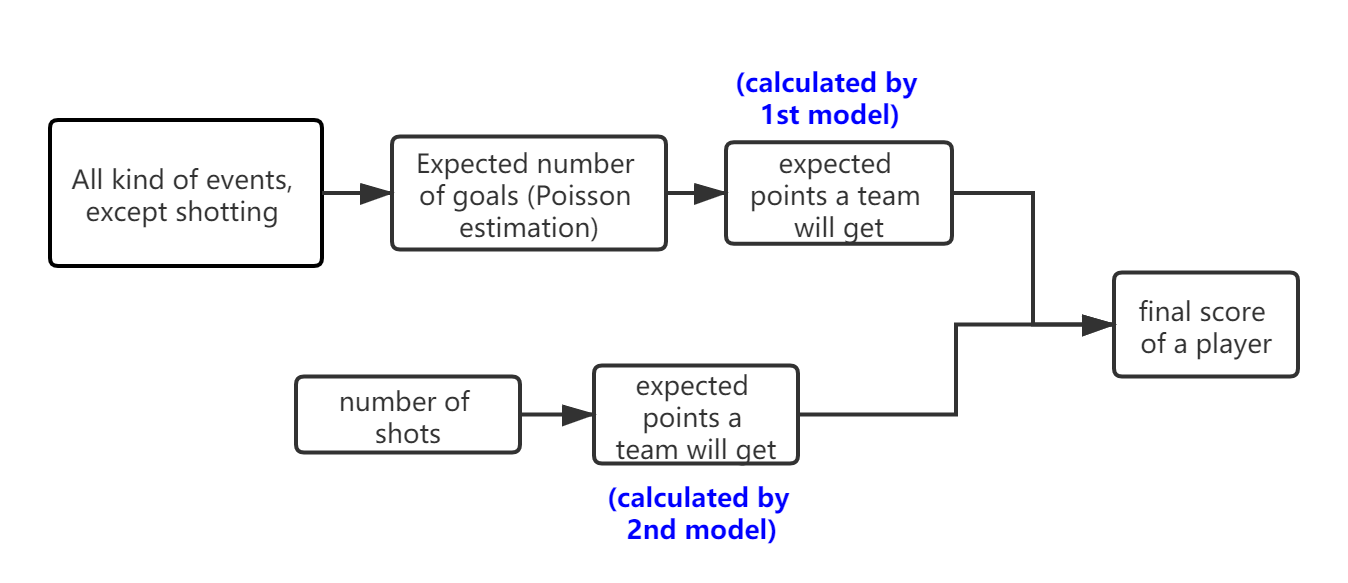
\includegraphics[width=0.9\textwidth]{flowchart_score.png}
	\caption{The Flow Chart of the Rating Process}
	\label{fig:flow_score}
\end{figure}

The contribution of a player can be accurately calculated by assessing how his behaviour influences the final point the team gets in the match(for instance, 3 points if the team wins). But the point itself is difficult to simulate directly, so we instead try to research how the all kinds of events happening on the field influence the number of goals in one game.

To simplify the model, we assume the shot number of each game as independent Poisson variables, with a stable "scoring rate" (that is, the possibility of scoring a goal) ~\cite{development}. That it to say,
\begin{equation}
P(X_t=k) = e^{-\lambda t} \frac{(\lambda t)^k}{k!}
\end{equation}

All the events that may contribute to making a shot are called "positive events"(or posEvent for short) and the opposite ones are called "negative events"(or negEvents for short). And the contribution is calculated with a linear model.

\begin{equation}
\begin{aligned}
E_{sh} &= \sum{\alpha _i N_{Ph,i}} - \sum{\beta _j N_{Na,j}}\nonumber\\
E_{sa} &= \sum{\alpha _i N_{Pa,i}} - \sum{\beta _j N_{Nh,j}}\nonumber
\end{aligned}
\end{equation}

where 

\begin{itemize}
	\item $E_{sh}$ is the expected number of shots made by the home team in one game, while $E_{sh}$ is the expected number of shots by the away team.
	\item $N_{Ph,i}$ is the number of $posEvent_i$ conducted by the home team, while $N_{Pa,i}$ is the number of $posEvent_i$ conducted by the away team. The positive events may refer to a successful pass,a crossing, etc.
	\item $N_{Nh,j}$ is the number of $negEvent_j$ conducted by the home team, while $N_{Na,j}$ is the number of $negEvent_j$ conducted by the away team. The negative event may refer to an unsuccessful pass, a red card received by a team member, etc
	\item $\alpha _i$ is called coefficient of $posEvent_i$, while $\beta _i$ is called coefficient of $negEvent_i$
\end{itemize}

To find out the coefficients of each events, a linear regression is needed. But because of the limit of data, we refer to the coefficients used in the rating model implemented by EA Sports Player Performance Index~\cite{development} instead, and the specific value can be consulted in the paper~\cite{development} .

The expected number of goals made in a game is
\begin{equation}
\begin{aligned}
E_{gh} &= pE_{sh}\nonumber\\
E_{ga} &= p^{'}E{sa}\nonumber
\end{aligned}
\end{equation}
$E_{gh}$ is the expected number of goals made by the home team, and $E_{ga}$ is the expected number of goals made by the away team. $p$ and $p^{'}$ are "shooting conversion rate" that may be influenced by different counterparts. In the simple case, we may treat them as a constant.
\begin{equation}
\begin{aligned}
E_{PTS} &= (3\ points) \times (possibility\ of\ a\ win) + (1\ point) \times (possibility\ of\ 					a\ tie)\\
&= (3\ points) \times (p_{(1:0)} + p_{(2:0)} + p_{(2:1)} \cdots + (1\ points) \times 
(p_{(0:0)} + p_{(1:1)} \cdots)\\
&= exp(- E_{gh} - E_{ga}) \{3\sum_{i=1}^{\infty}{\sum_{j=i+1}^{\infty}{\frac{E_{gh}^j E_{ga}^i}{i!j!}}} + \sum_{i=1}^{\infty}{\frac{E_{gh}^i E_{ga}^i}{i!i!}}\}
\end{aligned}
\end{equation}

$E_{PTS}$ is the expected number of points that the home team gets. The value of a single event can be calculated by $\partial E_{PTS} / \partial N_i$, where $N_{i}$ is the number of event i. In this way, we could calculate the performance score of each member by summing up all the value of events conducted by him.

The model has a drawback that it fails to find out the significance of shots. To polish up the model, we calculate the importance of shots in a slight different way. From the world-famous football statistic website 'whoscored'~\cite{score}, we can find out that a score is 'worth' about $1.03$ points in the tournament, and the average "scoring possibility" of a a shot is around $12.4\%$. So a shot is actually worth about $1.03 * 12.4\% = 0.128$ point to the team. 

And the final score of a player can be calculated by adding up the value of all common behavior and shooting conducted by a player in a game with a coefficient, which helps make the highest score no more than 100.
\begin{figure}[h]
	\centering
	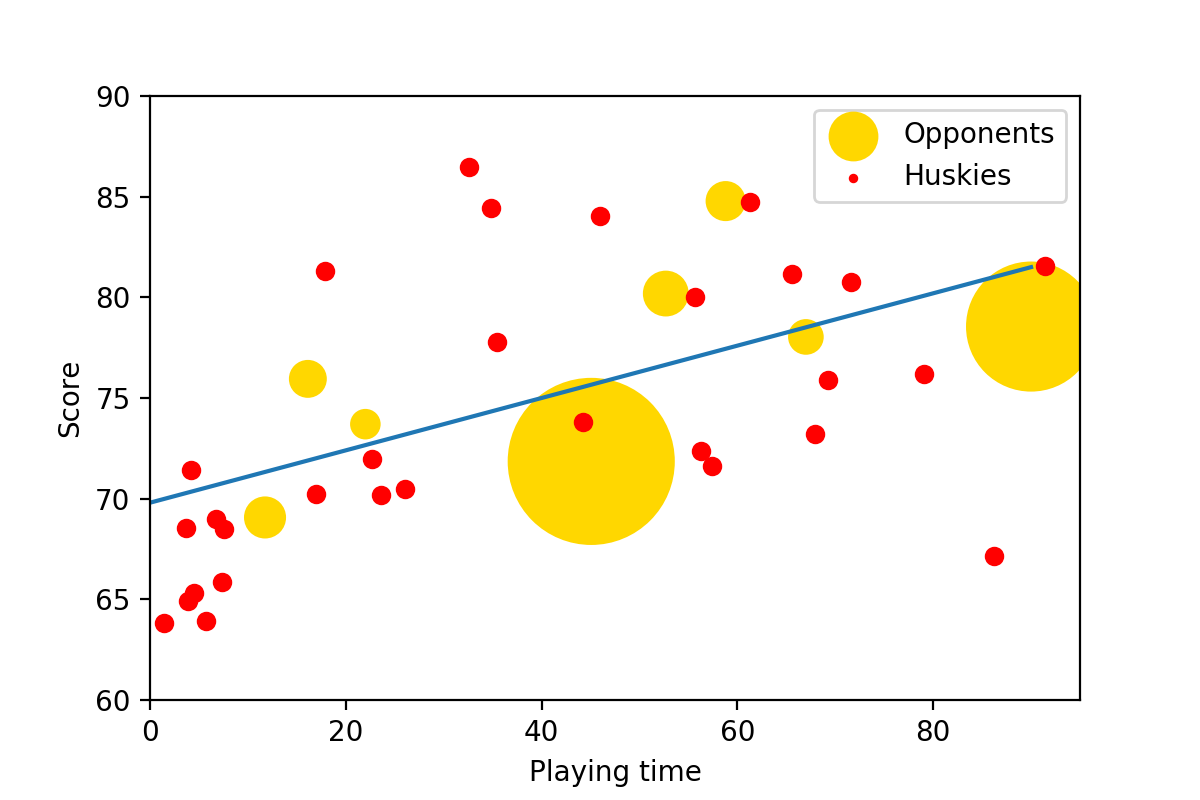
\includegraphics[width=0.45\textwidth]{scoreplot.png}
	\caption{Relationship Between Playing Time and Score of Each Player}
	\label{fig:score_plot}
\end{figure}

The result of the model can be found in \ref{fig:score_plot}. For red dots, the x-axis coordinate shows the average playing time of each Huskies player, and the y-axis coordinate shows the score of the player. While the x-axis coordinate of yellow dots represent the same thing as red dots, the y-axis coordinate of the yellow dots represents the average score of opponent players whose average playing time is in this interval, and the size of yellow dots represents the number of opponent players with average playing time in such interval.  We can find that the scores Huskies players get are roughly the average in the league. Moreover, the Huskies players who own more playing time do play a little better than the bench players, though the difference is not so obvious.

	An the specific scores of each member of the Huskies team are listed in the 'Implementation' section.

\subsection{Ways to Analyze Indicators}
	We use \textbf{Analytic Hierarchy Process (AHP)} and \textbf{Principal Component Regression (PCR)} to analyze these indicators and get the results of team performance.
	
	\paragraph{AHP}
	In order to build a model about teamwork and level based on the indicators mentioned above, we use \textbf{Analytic Hierarchy Process (AHP)} to allocate the weight of different indicators.
	
	AHP is multiple criteria decision-making tool. This is an Eigen value approach to the pair-wise comparisons. AHP can help us determine the weight of each factor.~\cite{analytic} The procedure for using the AHP ~\cite{ahp} can be summarized as:
	\begin{enumerate}
		\item Model the problem as a hierarchy which contains the decision goal, the alternatives for reaching it, and the criteria for evaluating the alternatives.
		\item Establish priorities among the elements of hierarchy by making many judgments based on pairwise comparisons of the elements.
		\item Synthesize these judgments to produce overall priorities for the hierarchy.
		\item Check the consistency.
		\item Come to a final decision based on these judgments.
	\end{enumerate}

	In step (2), we need to build consistency matrix to compare every two elements. The element $e_{i, j}$ in the matrix is defined as:
	\begin{itemize}
		\item 1, if $i$ and $j$ are similarly important;
		\item 3, if $i$ is slightly important than $j$;
		\item 5, if $i$ is apparently important than $j$;
		\item 7, if $i$ is intensively important than $j$;
		\item 9, if $i$ is extremely important than $j$;
		\item 2, 4, 6, 8, the middle value of the importance above;
		\item reciprocal, $a_{j, i}= \frac{1}{a_{i, j}}$.
	\end{itemize}
	
	We then calculate the max eigenvalue $\lambda$ of the matrix and the eigenvector of $\lambda$. The normalization of this eigenvector is written down as $W$. The elements in $W$ is the weights of criteria. After that, we calculate \textbf{Consistency Index (CI)} and \textbf{Random Index (RI)} to check our results.~\cite{analytic}
	
	In our model, our decision goal is team performance. As is shown in Figure \ref{fig:ahp}, $L_0$ represents the goal layer. $L_1$, $L_2$, $L_3$, and $L_4$ represent criteria layer. $W_1$, $W_2$, \ldots, $W_7$ represent normalized eigenvectors of max eigenvalue of consistency matrix. $M_1$, $M_2$, \ldots, $M_9$ are metrics mentioned in ``Indicators of the Whole Team'' \textit{in the same order}. After calculating all of eigenvectors mentioned above, we could have the final weight of these indicators, in terms of both the whole team and every player.
	\begin{figure}[h]
		\centering
		\includegraphics[width=0.8\textwidth]{ahpnew.pdf}
		\caption{AHP Diagram of Our Model}\label{fig:ahp}
	\end{figure}
	
	\paragraph{PCR}
	We can also use the \textbf{Principal Component Regression (PCR)}, which uses \textbf{Principal Component Analysis (PCA)} and regression, to analyze the possibility that the football team win a match or not.
	
	The basic idea of PCA is mapping n-dimension features onto k-dimension. The newly formed k-dimensional features are orthogonal, which are called ``principal component''. We could calculate the coefficient matrix of the original matrix and select $k$ eigenvectors whose eigenvalues are the maximum among all eigenvalues. Therefore, we could get new data matrix based on these $k$ eigenvectors.~\cite{principal}
	
	In our model, we use PCA to convert 9 metrics (9 dimensions) which are mentioned in ``Indicators of the Whole Team'' into 3 new features(3 dimensions). After PCA, we apply common regression analysis in our new data matrix and investigate in the results. 
	
\subsection{Implementation of Our Performance Model}
\subsubsection{Results of Team Metrics and Players' Ratings}
	After calculation, we got results of 9 metrics that can indicate something about Huskies team. We list them in Table \ref{tab:metrics}. The detailed data could be found in Appendix (). \textit{Notice that} \textit{Pagerank Variance ($\sigma ^2$) is the variance of pagerank $x_i$ in 38 matches. Other metrics are the average numbers in 38 matches.}
	
	\begin{table}[h]
		\centering
		\caption{Nine Metrics of Huskies Team}
		\label{tab:metrics}
		\begin{tabular}{|c|c|c|c|c|}
			\hline
			Closeness ($\bar C$) & Betweenness ($\bar C_B$) & Pagerank Variance ($\sigma ^2$) & Clustering ($\bar c$) & x-axis of Centroid ($\bar M_x$)\\
			\hline
			0.6889&
			0.03832&
			0.0005988&
			0.6645&
			49.98\\
			\hline
		\end{tabular}
		\begin{tabular}{|c|c|c|c|}\hline
			The Shortest Attack Path ($\bar P$)  &The Maximum Flow ($\bar |f|$) &  Edge Connectivity ($\bar N_e$) & Passing Times ($\mu$)\\
			\hline
			0.4607&
			4.108&
			1.605&
			275.0\\
			\hline
		\end{tabular}
	\end{table}
	The rating model gives us a distinct view of how well a player performs in the team and this is also an important aspect of the performance of the whole team. We calculate the rating score of each player in Huskies team based on our rating model and list scores in Table \ref{tab:score}. The score could range from 60 to 100. Players' IDs are shown in odd columns.
	\begin{table}[h]
	\centering
	\caption{Rating Scores of Players in Huskies Team}
	\label{tab:score}
	\begin{tabular}{|c c|c c|c c|c c|c c|c c|}
		\hline
		G1 &67.16 &F1 &73.8 &F2 &80.77 &F3 &68.5 &F4 &71.97 & F5 & 70.5\\
		F6 &86.49&M1&81.54&M2&65.86&M3&73.23&M4&71.64&M5&68.55\\	
		M6&81.18&M7&63.83&M8&70.19&M9&	70.22&	M10&65.33&M11&63.9\\
		M12&81.32&M13&69.01&D1&76.19&D2&72.38&D3&75.88&D4&80.02\\	
		D5&84.72&D6&77.79&D7&84.03&D8&	84.45&D9&71.42&D10&64.9\\
		\hline
	\end{tabular}
	\end{table}
\subsubsection{Results of AHP and Weight Vector}
	We set every consistency matrices based on the comparison of importance between two indicators. If we use $W_1$, $W_2$, \ldots, $W_7$ to represent eigenvectors mentioned above and use $A_1$, $A_2$, \ldots, $A_7$ to represents consistency matrix, then we have:
	\begin{equation}\nonumber
	\begin{aligned}
		&A_1 = 
		\begin{bmatrix}
		1&\frac{1}{2}\\
		2&1
		\end{bmatrix}
		\text{, }
		W_1 = 
		\begin{bmatrix}
		\frac{1}{3}\\
		\frac{2}{3}
		\end{bmatrix}
		\text{, }
			A_2 = \begin{bmatrix}
		1 & \frac{1}{3}\\
		3&1
		\end{bmatrix}
		\text{, }
		W_2 = 
		\begin{bmatrix}
		\frac{1}{4}\\
		\frac{3}{4}
		\end{bmatrix}
		\text{, }
			A_3 = \begin{bmatrix}
		1 & \frac{1}{2}\\
		2&1
		\end{bmatrix}	
		\text{, }
		W_3 = 
		\begin{bmatrix}
		\frac{1}{3}\\
		\frac{2}{3}
		\end{bmatrix}
		\text{, }
			A_4 = \begin{bmatrix}
		1 & 1\\
		1&1
		\end{bmatrix}
		\text{, }
		W_4 = 
		\begin{bmatrix}
		\frac{1}{2}\\
		\frac{1}{2}
		\end{bmatrix}
		\text{, }
		\\
			&A_5 = \begin{bmatrix}
		1 & \frac{1}{3}& \frac{1}{3}\\
		3&1&1\\
		3&1&1
		\end{bmatrix}
		\text{, }		
		W_5 = 
		\begin{bmatrix}
		\frac{3}{5}\\
		\frac{1}{5}\\
		\frac{1}{5}
		\end{bmatrix}
		\text{, }
			A_6 = \begin{bmatrix}
	1&	1&	\frac{1}{3}&	\frac{1}{5}\\
	1&	1&	\frac{1}{3}&	\frac{1}{5}\\
	3&	3&	1&	1\\
	5&	5&	1&	1
		\end{bmatrix}
		\text{, }
		W_6 = 
		\begin{bmatrix}
		0.10	\\0.10\\	0.35\\	0.45
		\end{bmatrix}
		\text{, }
		A_7 = \begin{bmatrix}
		1 & 1&1\\
		1&1&1\\
		1&1&1
		\end{bmatrix}
		\text{, }
		W_7 = 
		\begin{bmatrix}
		\frac{1}{3}\\\frac{1}{3}\\\frac{1}{3}
		\end{bmatrix}
	\end{aligned}
	\end{equation}
	
	If we use $W$ to represent \textit{the final weights} of nine metrics and the players' scores of our rating model, then we calculate elements in vector $W$:
	\setcounter{MaxMatrixCols}{20}
	\begin{equation}\nonumber
		W = 
		\begin{bmatrix}
		0.111&
		0.111&
		0.111&
		0.0556&
		0.111&
		0.15&
		0.05&
		0.05&
		0.0255&
		0.0255&
		0.0869&
		0.112&	
		\end{bmatrix}
		^T
	\end{equation}
	
	The elements in the vector are the weights of \textit{forward score, midfield score, defend score, passing times, x-axis of centroid, the shortest path, the maximum flow, connectivity, betweenness, closeness, pagerank, and clustering }respectively.
	
	We normalize all the factors involved before implementing AHP to make the process more sensible. 
	
	We can use $W$ and the data of these indicators to calculate a final score of Huskies team. The final score indicates the performance of the whole team. If we compare this score with another team's score, we can possibly predict the result of match. We calculate AHP score of four matches: 
	\textbf{match 5, 0.497, lose; match 14, 0.600, win; match 18, 0.519, win; match 23, 0.441, lose.} The AHP scores of wining matches is higher than scores of losing matches, which verifies the correctness of our AHP model and $W$.
	
\subsubsection{Results of PCR}
	We use PCA algorithm in Python and do regression based on nine metrics of the whole team. First, we use PCA to reduce the dimensions into three and plot 38 matches in Figure \ref{fig:pca}. From Figure \ref{fig:pca}, it can be concluded that we can distinguish the results of matches easily when we reduce dimensions of metrics into three. These three new dimensions may not have the actual meanings but can help us classify the results.
	\begin{figure}[h]
		\centering 
		\begin{subfigure}[b]{0.32\textwidth}
			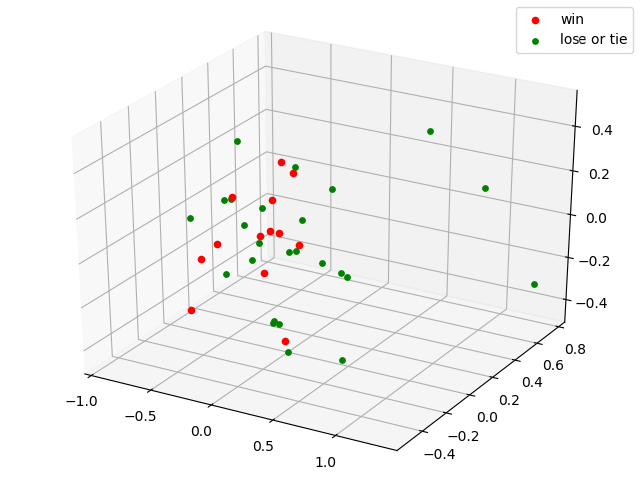
\includegraphics[width=\textwidth]{win_or_not_win.png}
			\caption{}
		\end{subfigure}
		\begin{subfigure}[b]{0.32\textwidth}
			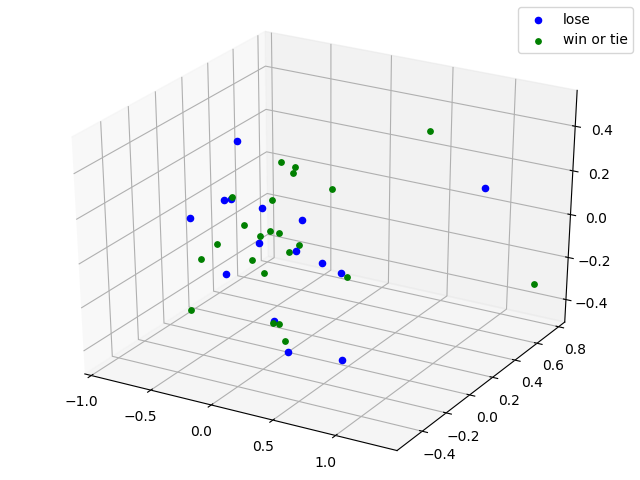
\includegraphics[width=\textwidth]{loss_vs_not_loss.png}
			\caption{}
		\end{subfigure}
		\begin{subfigure}[b]{0.32\textwidth}
			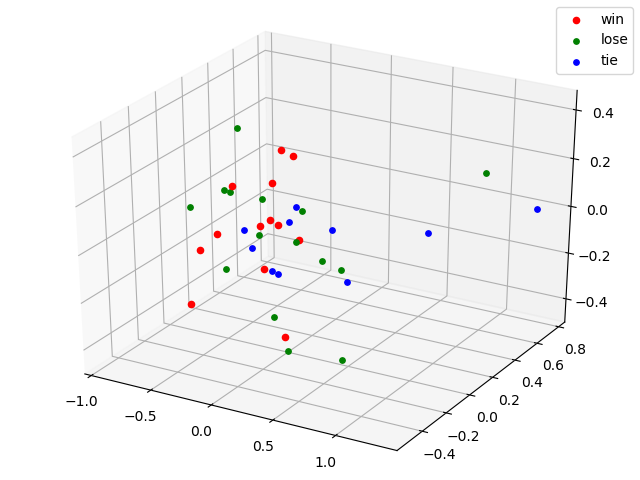
\includegraphics[width=\textwidth]{win_vs_lose_tie.png}
			\caption{}
		\end{subfigure}
	\caption{PCA Results (a) shows the distribution of win and ``lose or tie'' in 3 dimensions space; (b) shows the distribution of lose and ``win or tie'' in 3 dimensions space; (c) shows the distribution of win, tie, and lose in 3 dimensions space.}
	\label{fig:pca}
	\end{figure}

	We also reduce the dimensions into two and try to do linear regression with 2 new features. As is shown in Figure \ref{fig:regression}, we use PC1 and PC2 to represent two new features and the third dimension is the score of $performance$ that Huskies team get in every match. We plot a fitting plane in our figure. We can discover that in Figure \ref{fig:regression} (a), the plane may not fit the points well, while in Figure \ref{fig:regression} (b), the plane fits the points well. The result indicates that two-dimensional features may lose a bit of information and need further investigation.
	\begin{figure}[h]
		\centering
		\begin{subfigure}[b]{0.4\textwidth}
			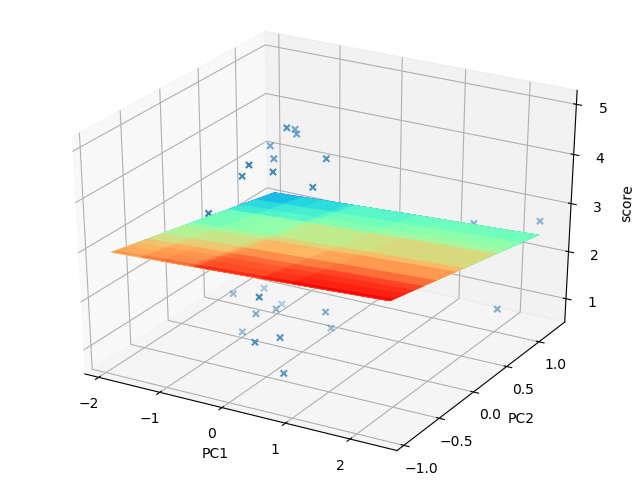
\includegraphics[width=\textwidth]{PCA2.png}
			\caption{}
		\end{subfigure}
		\begin{subfigure}[b]{0.4\textwidth}
			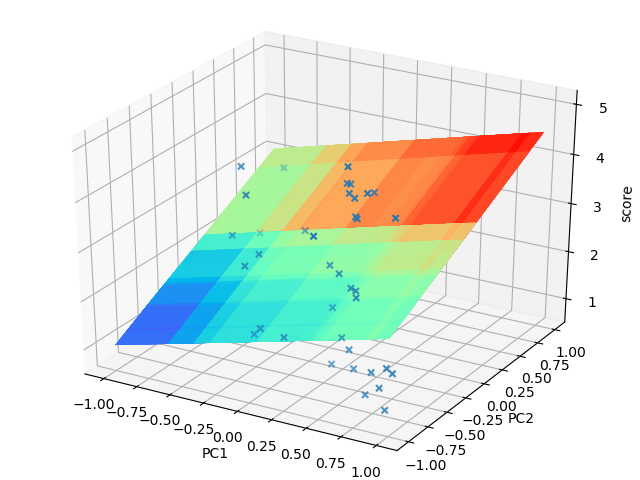
\includegraphics[width=\textwidth]{PCA.png}
			\caption{}
		\end{subfigure}
	\caption{Regression Results (a) does regression with 2 features PC1 and PC2 that our former PCA  process gets; (b) does regression with randomly selected two features PC1 and PC2 among nine metrics of the whole team}
	\label{fig:regression}
	\end{figure}
\section{Possible Stratigies for Huskies Team}
\subsection{Current Performance of Huskies Team}
Some structural strategies that Huskies currently adopted have been effective in matches and are reflected on the passing network and performance model.

From the passing network, we could find out that Huskies team has build a relatively closely connected passing network from goalkeeper to forwards. We suppose the team applied a \textbf{5-4-1 formation} in the last season. By calculating the number of triangles and the number of shots, we could discover that Huskies can organize threatened attacks and cooperate closely. When the team loses a score, players are good at pass the ball back and look for a chance to strike back. And the pass distribution has shown that the team is good conducting long passes across the field to mobilize opponents' defence line, which is a wise strategy. However, compared with opponents, Huskies has fewer chances to pass the ball forward, and is forced to pass only in the backfield. It may explain the unsatisfying score of the team in the last season.

From the performance model, we could find out that the ratings of most players are average or above average, and higher rated players have more playing time. Apart from that, 9 metrics indicate that the performance whole team is not so bad, though further improvement is expected.
\subsection{Strategies of Matching Style}
From the average positions of players, we could find out that the positions of some forwards  midfielders are in Huskies team's half field. As result, we suggest forwards and midfield players be \textbf{more aggressive} and try to run in opponent's half field to find more chance to attack and take a shot. The 5-4-1 formation has one forward, so we suggest the team should add forwards to the starting line-up.

From passing network, we suggest Huskies team should \textbf{reach a balance} between attack and defense. The players are more accustomed pass the ball backward rather than forward. Passes in the backfield are very well-organized but they lack passes in the front field. Pass the ball in the front filed more often, form more triangles, and it will bring more shots and more goals.

\subsection{Strategies of Training Players}
Based on our rating model, we find that the player F6 gets the highest score of rating (86.49). He participated in the game after the 24th match. After his joining, the performance of Huskies improved, and it won 6 of 13 matches, with 3 ties. He deserves more playing time. The average rating score of forward, midfields, and defends of Huskies team are 73.11, 71.22 and 77.19 respectively. In contrast, those of opponent team are 69.24, 76.50, 76.58. Therefore, we suggest Huskies \textbf{make improvements in its midfield}. Considering the rating and players' positions, we put forward our dream team of Huskies current players in Figure \ref{fig:team}.
\begin{figure}[h]
	\centering
	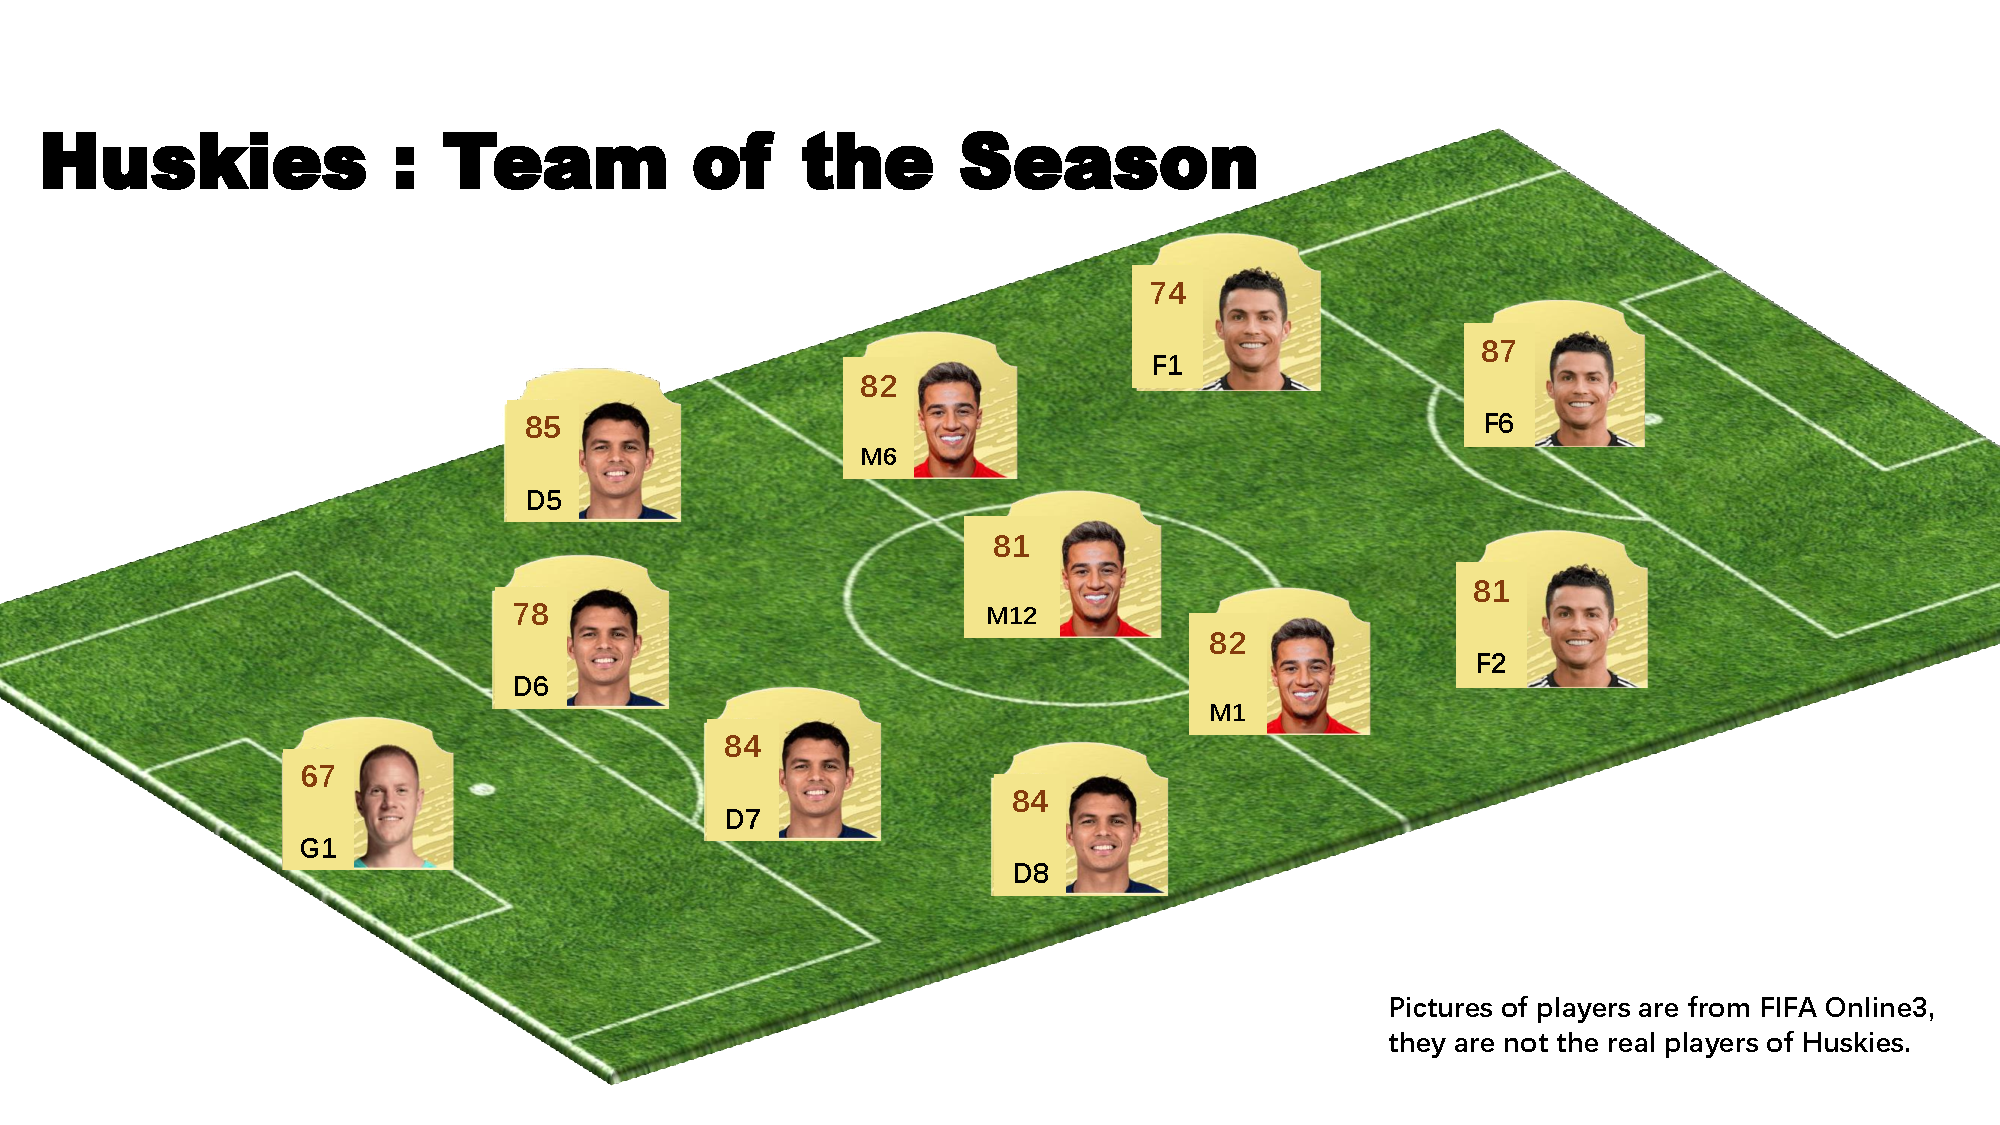
\includegraphics[width=0.6\textwidth]{best.pdf}
	\caption{Dream Team of Huskies}
	\label{fig:team}
\end{figure}

\subsection{Strategies of Improving Cooperation}
We have calculated the weight vector $W$. Thereby, we could choose 3 most important indicators whose weights are more than others. The 3 chosen indicators are: \textbf{x-axis of centroid (0.111)}, \textbf{the shortest path (0.15)}, and \textbf{the clustering (0.112)}. Huskies team needs to improve these aspects especially.

In terms of x-axis of centroid, it reflects the general style of team, such as defend style and attacking style. As a result, all players need run ahead and pass the ball ahead, not just pass the ball in the midfield. They need to organize more times of attack and put the centroid forward.

In terms of the shortest path, the players need to pass the ball precisely and safely and avoid being cut by the opponent players. Besides, they also need to receive the passing ball wisely and think about how to deal with it, either passing it away or dribbling and have a shot. In this way, the cost of an attack will be smaller and increase the score of the shortest path.

In terms of clustering, players need to practice cooperation and try to form more triangles or quadrilaterals. Then, the players could pass the ball more easily because all players are connected closely.
\section{Further Study and Generalization of Model}
Besides application in the football field, the results of our research can also applied to other areas. 

\paragraph{Team Spirit}
In the fierce competition, the team needs to be aggressive and thirsty for winning. In another word, the team should possess a "winner temperament". Those who fear failure and fail to move forward will be defeated by the team who has seized every opportunity to win. Just as our discussion in Model 1, the Huskies team is more likely to win when they move their formation forward, and pass the ball firmly towards the opponents' goal.

\paragraph{Team member composition}
It is also important to have a group of outstanding team members. A balanced team is the base for success. On the contrary, the lack of good players in the midfield in Huskies may have actually caused the struggle in its attacking. But the 'star members' in a team also counts. Just as what the player labeled Forward6 do in our data. 
% WALCOTT!!!!!!!!!!!!!!!!!!!!!!!
Moreover, it is necessary to keep a competitive atmosphere in the team. According to our model, the members who won more playing time in the Huskies do play better than the bench players, but the gap is not so wide. That is a just good example, because the short gap will inspire the young players who still lack playing time and help the improvement of whole team through competition. 

\paragraph{Assignment flow}
To make the discussion and team work more fluently, cooperation is important. We can compare the passes in football to the delivering of assignments. Everyone in the team should do his part, and then pass the uncompleted task to the next team member. When the football team passes more, it is more likely to find the flaw in the defender's formation, and is more likely to deliver the ball to the right place in time and to give a critical strike. Similarly, when the flow of assignments become more fluent, the team will exchange their ideas with each other with higher efficiency. Thus they will have more chance to find the deficiencies in their current job and polish it up before too late. 

\paragraph{O Captain! My Captain!}
Considering the Pagerank and the Clustering we has studied of the passing network, we could conclude that it is necessary for a team to have a captain, who is the core member of the team. The whole team centralizes the all the 'passes' around him, and obeys his order when necessary. When something unexpected happens, the captain should be the one who takes most of the responsibility and inspire the team to keep working. 

However, when the centralization becomes too severe, it may lead to the obscurity of other members. As a result,  the flow of assignments will be damaged and the efficiency will become lower. So it needs to be balanced.
\section{Model Analysis}
\subsection{Sensitivity Analysis}
\subsubsection{Sensitivity Analysis of Rating Model}
In the Rating Model For Players, we evaluate the score of a player by adding up all the 'contribution-events'. However, it is possible that the influence of particular events on the number of shots can not be calculated precisely with a linear model. Moreover, the coefficient of each kind of behavior adopted in our paper is actually cited from the paper~\cite{development}. The coefficient may not suit the games in our data well. So it is necessary for us to make a minor change in the coefficients, and find out how the results change accordingly. 

The passing and interception (which means "stop the opponents' pass") are two events that are most common in the game. So we will change the coefficients of them. Moreover, the number of shots influences the results, too. So the coefficient that converts number of shots to the addend of the player score also needs to be analyzed. The results of the coefficient change are as follows:

\begin{figure}[h]
	\centering
	\begin{subfigure}[b]{0.32\textwidth}
		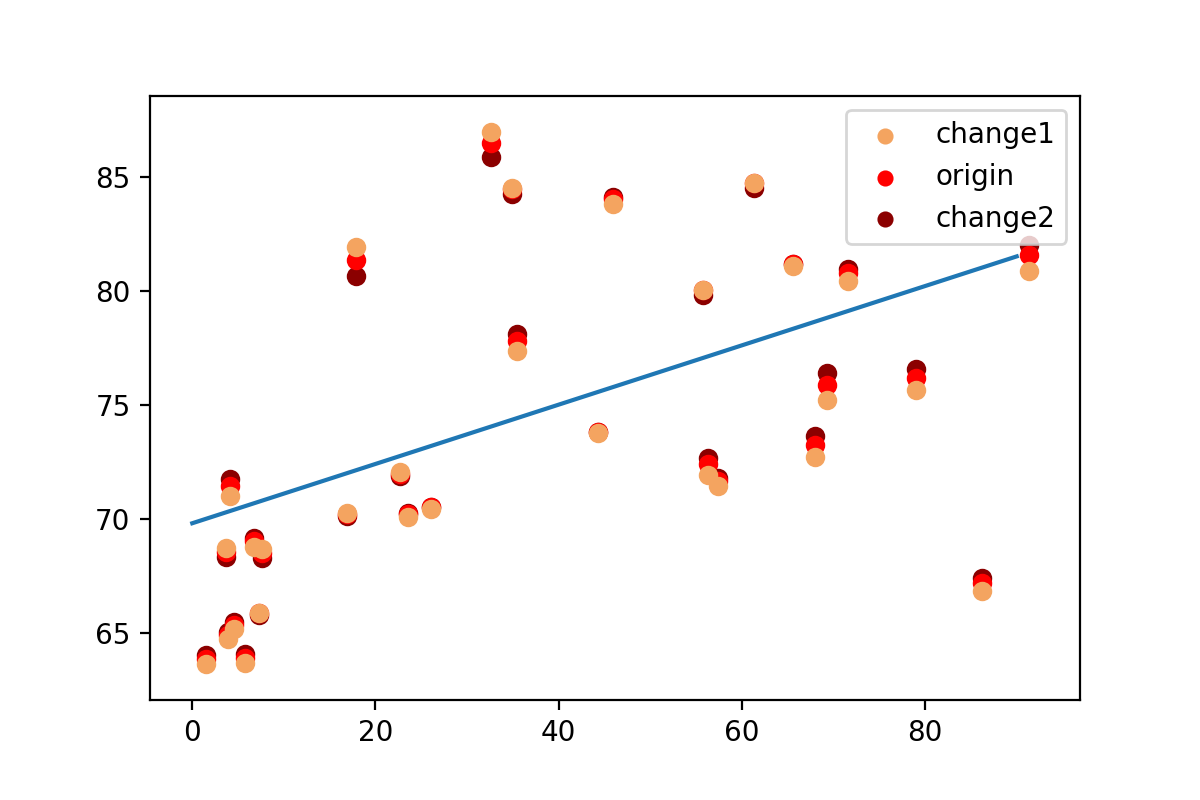
\includegraphics[width=\textwidth]{scoreplot_pass.png}
		\caption{}
	\end{subfigure}
	\begin{subfigure}[b]{0.32\textwidth}
		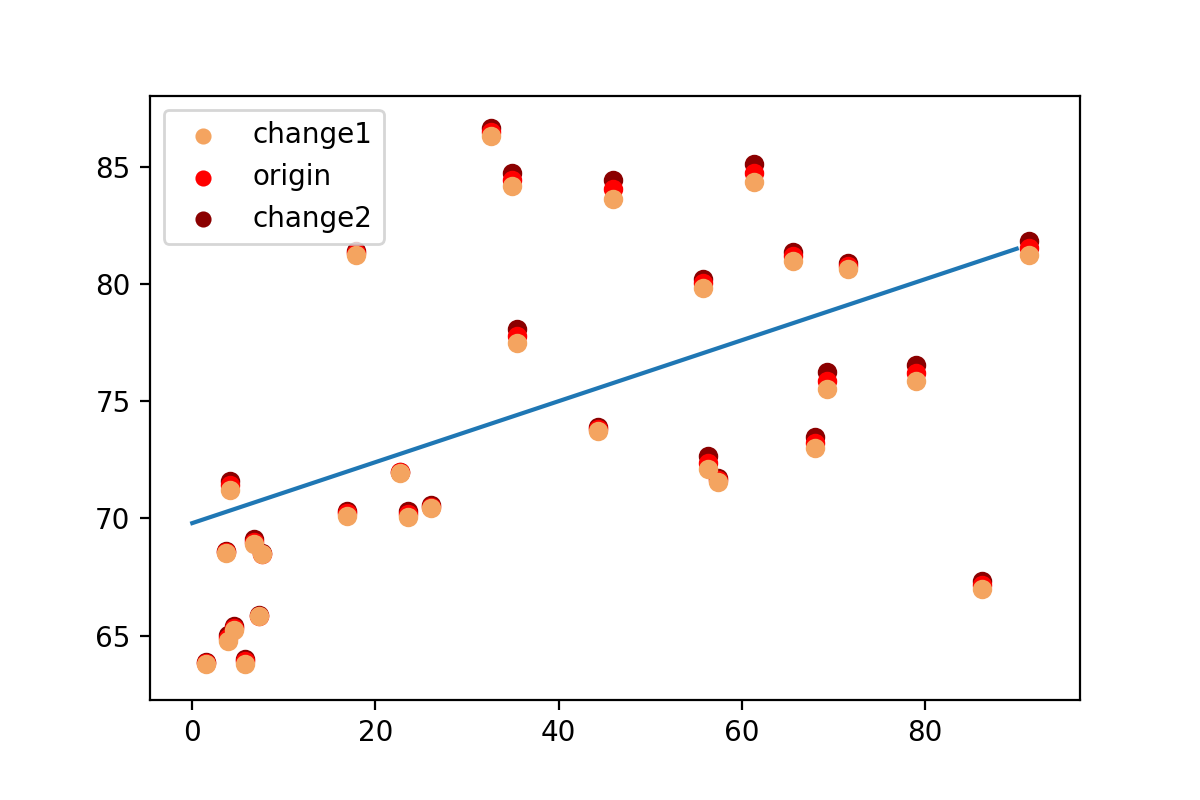
\includegraphics[width=\textwidth]{scoreplot_inter.png}
		\caption{}
	\end{subfigure}
	\begin{subfigure}[b]{0.32\textwidth}
		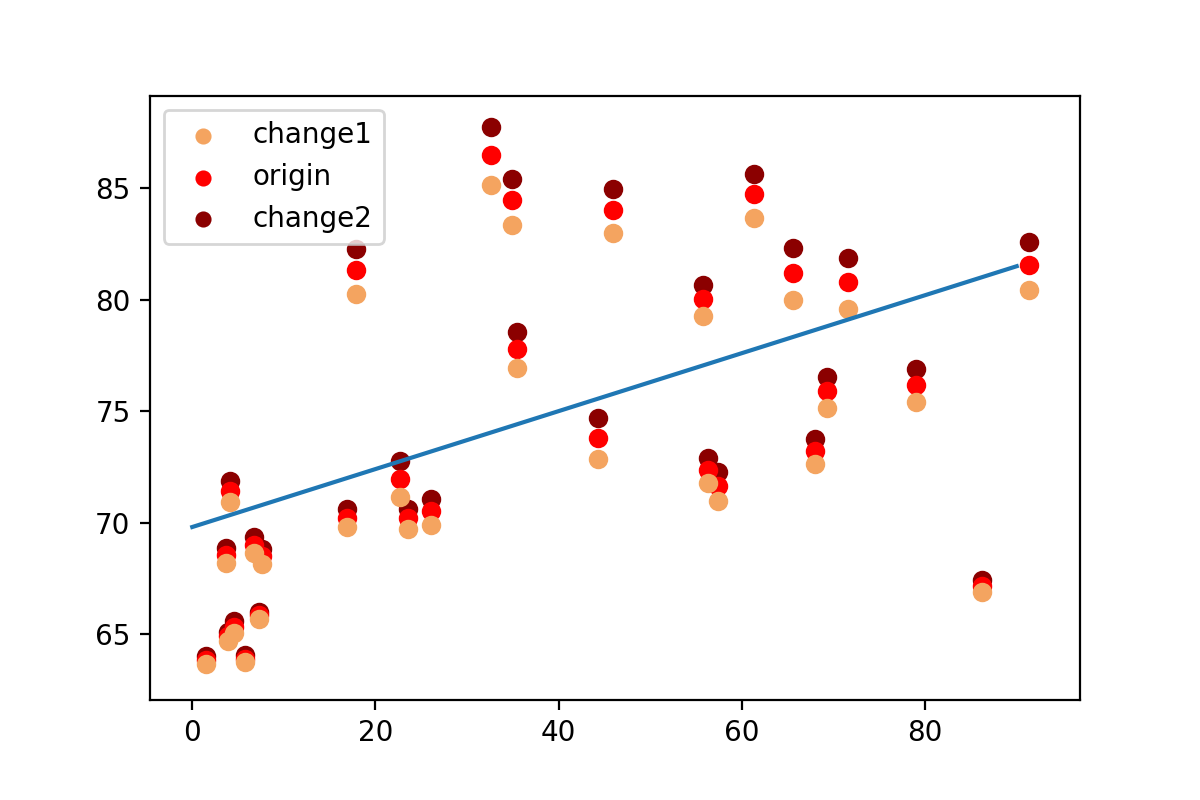
\includegraphics[width=\textwidth]{scoreplot_shot.png}
		\caption{}
	\end{subfigure}
	\caption{Changes of Huskies Players' Score When Changing Some of the Coefficients (a) is comparison by changing coefficients of passing; (b) is comparison by changing coefficients of interception; (c) is comparison by changing coefficients of shooting.}
	\label{fig:snsi_rate}
\end{figure}

In Figure\ref{fig:snsi_rate}, we decrease the coefficients in 'change1' by $10\%$,and increase the coefficients by $10\%$ in 'change2'. The changes for the location of the dots shows changes in the Huskies players' score.

When we change the coefficient of passing and interception in subfigure [a] and [b] , the final score of Huskies players are not greatly affected. The three dots nearly overlap. But when we change the coefficients for shooting, the differences are notable. So we take the situation into further analysis. The results are illustrated as follows:
\begin{table}[h]
	\centering
	\caption{Results After Changing Coefficients for Shooting}
	\label{tab:snsi_rating}
	\begin{tabular}{|c|c|c|c|c|c|}
		\hline
		&Origin score&Change1 Score& Changing Rate&Changes2 Score&Changing Rate\\
		\hline
		Average Change&$73.89$&$73.21$&$0.92\% $&$74.50$&$0.83\%$\\
		\hline
		Maximum Change&$86.49$&$85.13$&$1.58\% $&$87.72$&$1.42\%$\\
		\hline
	\end{tabular}
\end{table}

From the chart above, we can find that when we change the coefficient for shooting by $10\%$, the average score changes by less than $1\%$, and the maximum change is also well below $2\%$. It shows that our model is robust to the changes in the coefficients.

\subsubsection{Sensitivity Analysis of Team Metrics}
	As is shown in Figure \ref{fig:sens_team}, we randomly reduce the number of data to 95\%, 90\%, 85\%, and 80\% of the original data and calculate pagerank, closeness centricity, clustering, and betweenness centricity again. The four metrics fluctuate slightly around the original graph. In every subfigure, when the percentage of data decreases, the value decreases or increases in the same trend and does not have an extreme fluctuation. The results illustrate that our metrics model is robust to the change of data size.
\begin{figure}[h]
	\centering
	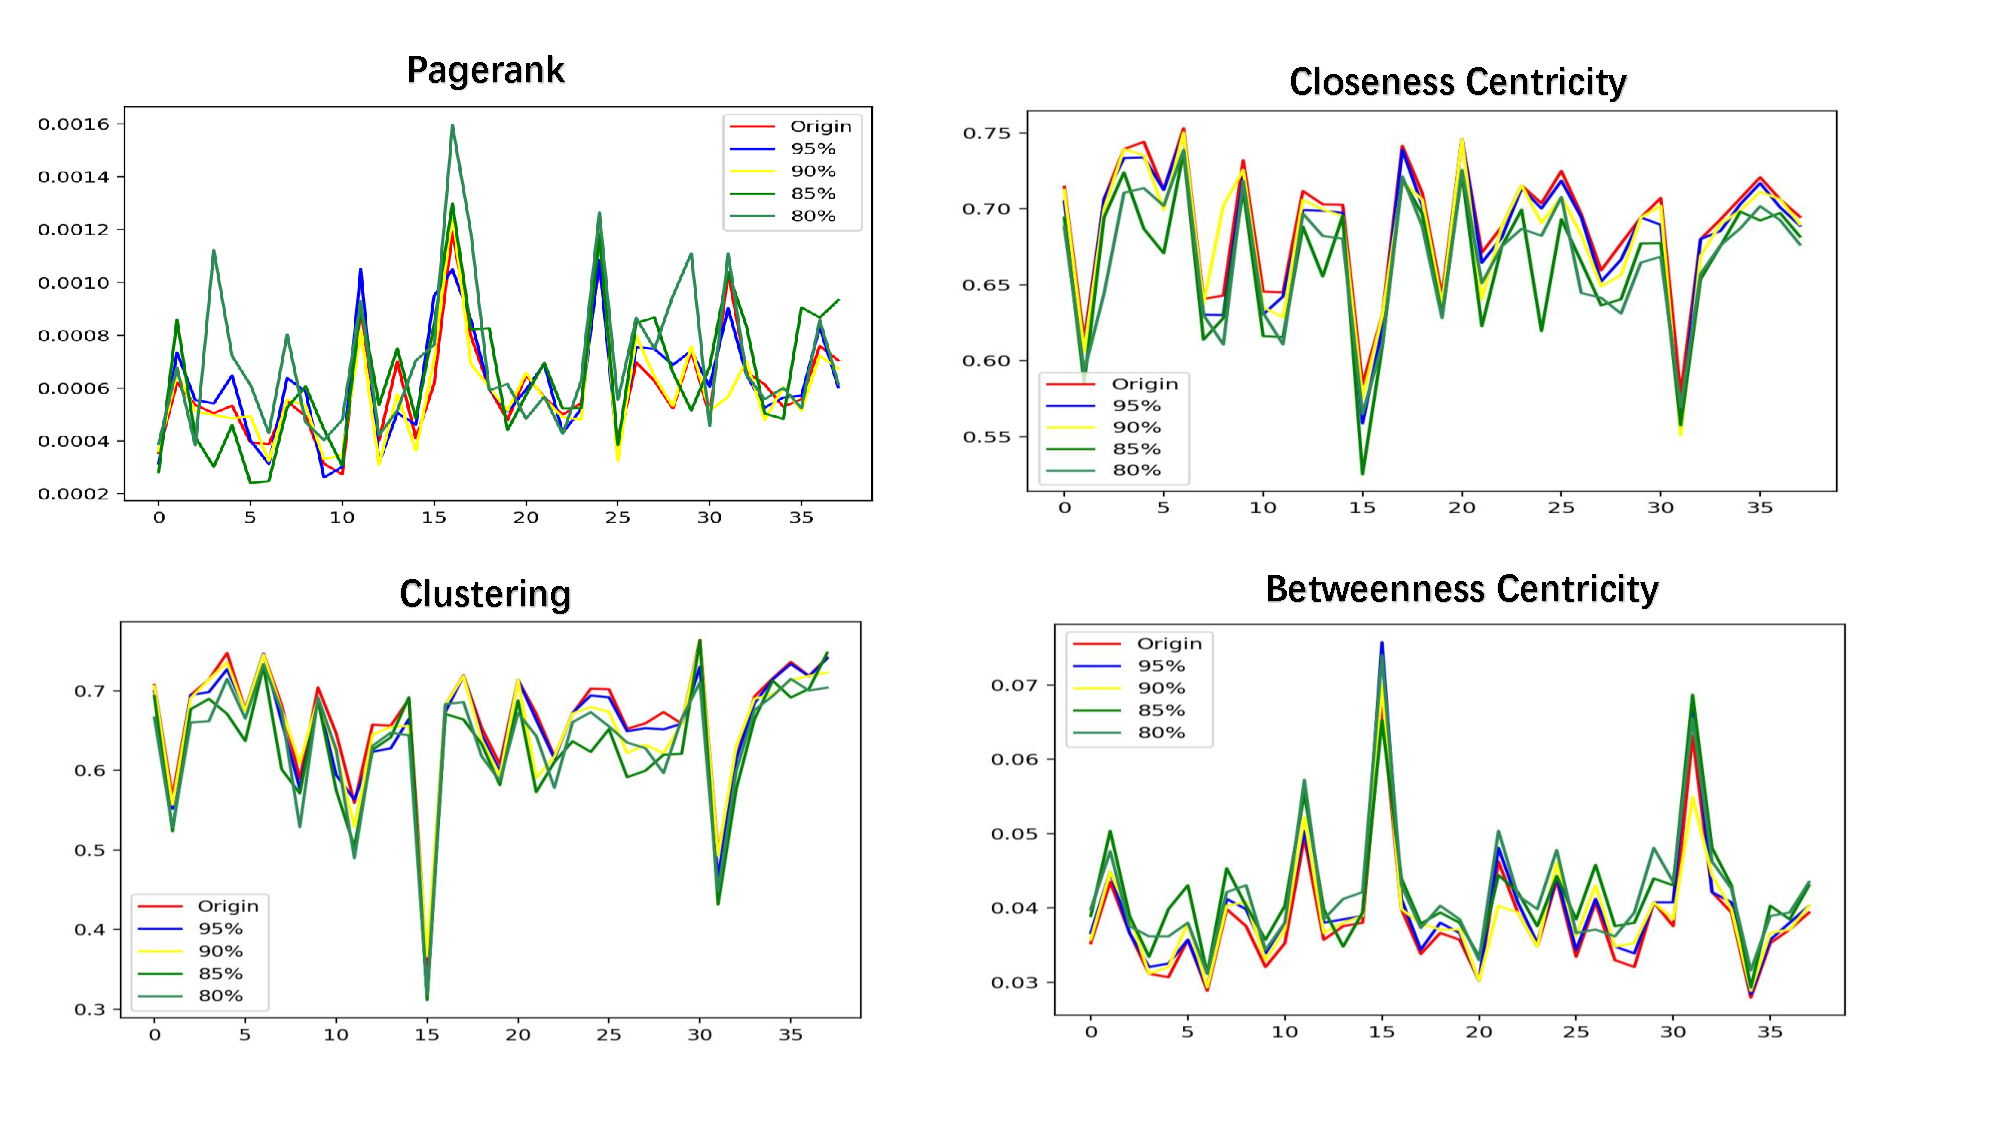
\includegraphics[width=\textwidth]{sens.pdf}
	\caption{Sensitivity Analysis of Four Team Metrics}
	\label{fig:sens_team}
\end{figure}
\subsection{Strengths and Weaknesses}
\subsubsection{Strengths}
	\begin{itemize}
		\item Our passing network model can reflect the actual passing events in the football fields. We can also find regular passing routes and attacking paths from the network clearly.
		\item Our nine metrics of the whole team can indicate different aspects of team performance and have particular meanings.
		\item Our rating model can rate every player's performance based on the events during the match and can compare their performance.
		\item Our AHP algorithm can mix indicators together and produce a general score that can help us assess team performance and cooperation. Our PCR algorithm can visualize and produce results.
		\item  Our model have a great robustness and can serve as original model of other cooperation events in our daily life.
	\end{itemize}
\subsubsection{Weaknesses}
	\begin{itemize}
		\item We do not have many data so the results of PCR are not so good.
		\item We only do research on one particular team. Therefore, our model needs to be further research and test.
	\end{itemize}
\section{Conclusion}
	Our paper provides a detailed research on analyzing and assessing the performance and cooperation of a football team. We first analyze the passing network and triangles in them to get a distinct insight into the current state of the team. After that, we put forward nine metrics to evaluate team performance and rating model to evaluate players' performance. Then we use AHP to analyze the weight of each model and finall get the weight vector $W$, we also use PCR to try to predict results of matches based on $performance$ and two new features.
	
	After getting results of our model, we make suggestions for players and the whole team on how to improve cooperation and perform better. We also generalize our model to put forward some advice on how to design more effective team in our daily life.
	
	We test the sensitivity of our model and discover that our model have a great robustness. We believe our model can be applied in football training and other aspects of real life.
\bibliographystyle{IEEEtran}
\bibliography{refs}

\newpage
\begin{appendices}
	\section{Network Visualization Code}
	\lstinputlisting[language=Python]{drawnet.py}
	\section{Metrics Calculation Code}
	\lstinputlisting[language=Python]{MetricsGenerator.py}
	\section{Rating Model Code}
	\lstinputlisting[language=Python]{scoreforhuskiesmembers.py}
	\section{AHP Code}
	\lstinputlisting[language=Python]{ahp.py}
	\section{Sensitivity Analysis Code}
	\lstinputlisting[language=Python]{SensitivitiesAnalysis.py}
	\section{Other Tools Code}
	\lstinputlisting[language=Python]{mtools.py}
\end{appendices}
\end{document}